\documentclass[a4paper,12pt,normalheadings,footexclude,headinclude,liststotoc,nochapterprefix,onecolumn,oneside,parskip,pointlessnumbers]{scrreprt}

\usepackage[utf8]{inputenc}
\usepackage[ngerman]{babel}
\usepackage[T1]{fontenc}
\usepackage{graphicx}
\usepackage{setspace,natbib}
\usepackage{natbib}
\usepackage{abstract,amsmath,amssymb}
\usepackage[notindex,nottoc]{tocbibind}  %Inhaltsverzeichnisse erstellen
\usepackage[labelsep=space,justification=centering]{caption}
\usepackage{remreset}
\usepackage[lined,commentsnumbered]{algorithm2e}

\usepackage{amsthm}
\newtheorem{mydef}{Definition}

\renewcommand{\familydefault}{\sfdefault}

%Helvetica
%\renewcommand{\familydefault}{\sfdefault}
%\usepackage{helvet}

\usepackage[table]{xcolor}
\usepackage{colortbl}
\usepackage{multirow}

\usepackage{longtable} 
\usepackage{array} 
\usepackage{ragged2e} 
\usepackage{lscape} 
\usepackage{multirow} 
\usepackage{booktabs} 

\usepackage{csvsimple}

\SetAlgorithmName{Algorithmus}{Algorithmenverzeichnis}

% Fussnoten
\usepackage{chngcntr}
\counterwithout{footnote}{chapter}

%\usepackage[Sonny]{fncychap.sty}
\setlength{\parindent}{0pt}
\newcommand{\url}{\;}

\topmargin -0.9cm
\textheight 24cm
\textwidth 14cm
\oddsidemargin 1.5cm
\footskip 1cm

\onehalfspacing        % anderthalbzeilig

\renewcommand{\sectionmark}[1]{\markright{\footnotesize \sffamily\slshape \thesection\ #1}}

%Kopfzeilendefinition
\usepackage[fit]{truncate}
\usepackage{fancyhdr}
\pagestyle{fancy}
\cfoot{}
\lhead{\slshape\leftmark}
\rhead{\thepage}       % Eintrag rechts oben in Kopfzeile

%Kopfzeilendefinition bei neuem Kapitel
\makeatletter
\renewcommand\ps@plain{
 \renewcommand\@oddfoot{}  %leere Fusszeile
  \let\@evenfoot\@oddfoot
  \renewcommand\@oddhead{\hfil \normalfont \textrm{\thepage}}
  \let\@evenhead\@oddhead}
\makeatother

%Spaltendefinition f\"{u}r Tabellen
\usepackage{array}

%Formelnummerierung
\makeatletter
\@removefromreset{equation}{chapter}
\makeatother
\renewcommand*{\theequation}{\arabic{equation}}

%Tabellennummerierung
\makeatletter
\@removefromreset{table}{chapter}
\makeatother
\renewcommand*{\thetable}{\arabic{table}}

%Abbildungsnummerierung
\makeatletter
\@removefromreset{figure}{chapter}
\makeatother
\renewcommand*{\thefigure}{\arabic{figure}}


\begin{document}
\newpage\thispagestyle{empty}\null\newpage
\pagenumbering{roman}  %r\"{o}mische Seitennummerierung

%Titelseite
\begin{titlepage}
\begin{sffamily}
\begin{center}
  {\Huge{\bf Auftragsannahme- und}}\\[0.5cm]
    {\Huge{\bf Lagerhaltungsentscheidungen}}\\[0.5cm]
  {\Huge{\bf bei auftragsbezogenen}} \\[0.5cm]
    {\Huge{\bf Instandhaltungsprozessen}} \\[3cm]
  {\huge Masterarbeit} \\[1cm]
  {\Large zur Erlangung des akademischen Grades \\
  \glqq Master of Science (M.Sc.)\grqq\;im Studiengang Wirtschaftswissenschaft} \\[8mm]
  {\Large der Wirtschaftswissenschaftlichen Fakult\"{a}t \\
  der Leibniz Universit\"{a}t Hannover} \\[2cm]
  {\Large vorgelegt von} \\[8mm]
  {\Large\bf Robert Matern} \\[5mm]
  {\Large geb. am 7. März 1987 in Tschimkent } \\[2mm]
  {\Large (Matrikel-Nr. 2798160)} \\[2cm]
  {\Large\bf Erstpr\"{u}fer: Prof. Dr. Stefan Helber} \\[6mm]
  {\Large Hannover, den 11. September 2015}
  \end{center}
  \end{sffamily}
\end{titlepage}
\newpage


% Inhaltsverzeichnis
\tableofcontents

%Abkürzungsverzeichnis
\chapter*{Abkürzungsverzeichnis}
\addcontentsline{toc}{chapter}{Abkürzungsverzeichnis}
\begin{table}[h!]
    \vspace*{-3mm}
    \hspace*{2mm}
  \renewcommand{\arraystretch}{1,5}
  \begin{flushleft}
    \begin{tabular}{lp{11.5cm}}  %hier die Spaltenausrichtung und Anzahl eintragen
        APS & Advanced Planning and Scheduling Systeme \\
        ATO & Assemble-to-Order (engl. Begriff für kundenindividuelle Fertigung mit standardisierten Komponenten)\\
        DLP			& Deterministisch-lineares Programm\\
        DP  			 & Dynamisches Programm zur Annahme von Aufträgen\\
        DP-storage		    & Dynamisches Programm zur Annahme von Aufträgen unter Beachtung von Lagerbeständen\\
        %GAMS 		& General Algebraic Modeling System\\
        GE & Geldeinheiten \\
        MRO & Maintenance-Repair-and-Overhaul (engl. Begriff für Instandhaltungsprozess)\\
     MTO & Make-to-Order (engl. Begriff für Auftragsfertigung) \\
     MTS & Make-to-Stock (engl. Begriff für Lagerfertigung)\\
     OK		    & Opportunitätskosten\\
     RM		    & Revenue Management\\
     SCM & Suppy Chain Management (engl. Begriff für Wertschöpfungslehre) \\
    u. B. d. R. & unter Berücksichtigung der Randbedingungen\\
	\end{tabular}
	\end{flushleft}
\end{table}

%Symbolverzeichnis
\chapter*{Symbolverzeichnis}
\addcontentsline{toc}{chapter}{Symbolverzeichnis}
\begin{table}[h!]
    \vspace*{-3mm}
    \hspace*{2mm}
  \renewcommand{\arraystretch}{1,5}
  \begin{flushleft}
    \begin{tabular}{lp{11.5cm}}  %hier die Spaltenausrichtung und Anzahl eintragen
    $\textbf{a}_{j}$ & Vektor des Ressourcenverbrauchs für Produktanfrage $j$\\
    $a_{hj}$ &	Verbrauch der Ressource $h$ für Produktanfrage $j$\\
   $\textbf{c}$ & Vektor der Ressourcenkapazität\\
   $c_{h}$ & Kapazität der Ressource $h$\\
    $D_{jt}$ & Aggregierte erwartete Nachfrag nach Produkt $j$ zur Periode $t$\\
    $h$	& Ressource aus der Menge $\mathcal{H}$\\
    $\mathcal{H}$ & Menge an Ressourcen\\
    $i$ & ... $\mathcal{I}$\\
    $\mathcal{I}$ & Gesamtmenge an möglichen Kombinationen ...\\
    $j$ & Produktanfrage aus der Menge $\mathcal{J}$\\
$\mathcal{J}$ & Menge an möglichen Produktanfragen \\   
$m$ & ... Ausführungsmodus aus der Menge $\mathcal{M}_{j}$\\
    $\mathcal{M}_{j}$ & Menge an produktspezifisch-möglichen Ausführungsmodi für ein Produkt $j$\\
 $\pi_{h}$ & Bid-Preis der Ressource $h$\\
   $p_{j}(t)$ & Wahrscheinlichkeit der Nachfrage nach Produkt $j$ in Periode $t$\\
    $r_{j}$ & Erlös des Produkts $j$\\
    $t$ & Periode des Buchungshorizonts $T$\\
        $\tau$ & Endperiode $t=1$ im Buchungshorizont $T$\\ 
        $T$ & Buchungshorizont\\
   $V(\textbf{c},t)$ & Ertragsfunktion in Abhängigkeit der Kapazitäten $\textbf{c}$ in der Periode $t$\\
    $x_{jm}$ & Anzahl der akzeptierten Anfragen nach Produkt $j$ im Ausführungsmodus $m$\\
	\end{tabular}
	\end{flushleft}
\end{table}






%Tabellenverzeichnis
\begingroup
\renewcommand*{\addvspace}[1]{}
\listoftables
\endgroup


%Abbildungsverzeichnis
\begingroup
\renewcommand*{\addvspace}[1]{}
\listoffigures
\endgroup


%\listofalgorithms
\newpage
\pagenumbering{arabic}   %ab hier arabische Seitenzahlen beginnend mit 1

\addcontentsline{toc}{chapter}{Vorwort}
\chapter*{Vorwort}
\markboth{Vorwort}{}


\chapter{Einleitung}
\markboth{1 Einleitung}{}

\section{Problemstellung}
%Unternehmen müssen aufgrund der heutigen dynamischen Veränderungen der Marktgegebenheiten die schnelle Entwicklung ihrer Produkte vorantreiben, sowie deren Platzierung und Bepreisung optimieren.\footnote{Vgl. \cite{gonsch2013using}, S. 94-95\label{dingens1}}
%Das Revenue Management (RM) ist daher für viele Dienstleistungsbereiche unabdinglich geworden. Durch dieses Managementkonzept und den daraus resultierenden Planungsinstrumenten können bei speziellen Anwendungsgebieten die Kapazitätsauslastungen optimiert werden. Damit lassen sich für Unternehmen mit Kapazitätsbe\-schränkungen die Absatzmärkte erfolgreich abschöpfen und die Gesamterlöse maximieren. In dieser Arbeit wird der Ansatz des Verkaufs von opaken Produkten im RM zur besseren Kapazitätsauslastung thematisiert. %\footnote{Klassische Ansätze des RM beschäftigen sich mit der Optimierung der Kapazitätsauslastung bei der Erstellung von Produkten oder Dienstleistungen.}
%Bei opaken Produkten handelt es sich um Produkte, bei denen der Anbieter einige Eigenschaften des Produkts bis zum Abschluss der Transaktion verbirgt.\footref{dingens1} %Anders als bei spezifischen Produkten, bei dem sämtliche Bestandteile der Produkteigenschaften vor dem Kauf bekannt sind.
%Die vorgestellten Produktarten werden i. d. R. in der Dienstleistungsindustrie von multiplen Anbietern angeboten.\footnote{Vgl. \cite{Klein:2008aa}, S. 4} Vereinfacht gesagt bedeutet dies, dass diese Anbieter ihre Dienstleistungen über eine Mehrmarkenstrategie distribuieren und ggf. ihr eigenes Produktportfolio mit anderen Dienstleistungen von Partnerfirmen erweitern. Sie bündeln aus dieser Menge an verfügbaren unterschiedlichen Dienstleistungen ein neues zusammenhängendes Produkt und vertreiben diese Art von Produkten über eine einzelne Marke an potentielle Konsumenten. Aus einem solchen Netzwerk an verfügbaren Produkten kann der Anbieter opake Produkte formen.\footnote{Vgl. \cite{anderson2009effectiveness}, S. 307-309}\textsuperscript{,}\footnote{Siehe Kapitel \ref{DP}}\\

Die Entscheidung über die Annahme von Kundenaufträgen hat weitreichenden Einfluss auf den Ertrag von produzierenden Unternehmen. Einem Unternehmen, dass zusätzlich zur Produktion auch die Instandsetzung ihrer Güter anbietet, steht vor dem Entscheidungsproblem, ob der Auftrag zur Instandsetzung des Gutes wirtschaftlich ist. Im weiteren Verlauf dieser Arbeit werden diese Unternehmen als sogenannter Instandhalter bezeichnet. Abhängig des eingehenden Kundenauftrags, indem der Zustand des Gutes beschrieben ist, durch den die notwendigen Prozessschritte zur Instandsetzung des Gutes abgeleitet werden können, generiert der Instandhalter unterschiedliche Erträge. Die Prozessschritte zur Instandsetzung des Gutes geben zusätzlich den notwendigen Ressourcenbedarf für die auszuführende Tätigkeit an, die notwendig sind um das Gut in seinen ursprünglichen bzw. geforderten Zustand zu versetzen. Ressourcen zur Instandsetzung von Gütern können z. B. Material oder Personalstunden sein.\footnote{Vgl. ... ???} Abhängig des möglichen Ertrags und des für den Auftrag notwendigen Ressourcenbedarf muss das produzierende Unternehmen die Entscheidung über Annahme oder Ablehnung des Kundenauftrags treffen. Sofern nur dieser einfache Fall betrachtet wird, bei dem nur der einzelne Kundenauftrag zur Auswahl steht, ist die Entscheidung für den Instandhalter einfach getroffen. Der Kundenauftrag wird angenommen, sofern der Aufwand des Ressourceneinsatzes niedriger als der erziele Ertrag ist (In dieser Arbeit wird auf eine differenzierte Betrachtung der Herstellkosten verzichtet).
Sofern der Unternehmen eine begrenzte Ressourcenkapazität zur Instandsetzung der Güter besitzt, muss zusätzlich der absolute Ressourcenverbrauch des Auftrags für Annahmeentscheidung geprüft werden. Mit Annahme des Auftrags ist ein auftragsbezogener Ertrag erzielt und ein produktbezogener Ressourcenverbrauch eingetreten. Nachdem diese Entscheidung getroffen ist, wird der zeitlich nachfolgende Kundenauftrag betrachtet.

Für die Entscheidung über die Annahme oder Ablehnung eines Kundenauftrags (KA) zur Instandhaltung von Gütern bedarf es einer umfassenderen Betrachtung, als nur die kurzsichtige Entscheidung über die Annahme einzelner Aufträge. Angenommen ein Instandhalter besitzt ein bestimmtes Kontingent an unterschiedlichen Ressourcen über einen bestimmten Zeitraum zur Erfüllung seiner angebotenen Dienstleistung. In diesem betrachteten Zeitraum treffen differenzierte Kundenaufträge mit unterschiedlicher Wertigkeit ein. Zur Maximierung der Erträge über diesen Zeitraum kann es für das Unternehmen sinnvoll sein Anfragen mit niedrigem Ertrag abzulehnen, sofern im weiteren Verlauf des betrachteten Zeitraums Aufträge mit höherem Ertrag eintreffen. Dies erfolgt in Abhängigkeit der noch vorhanden knappen Ressourcenkapazität.

Eine weitere Alternative wäre es für das instandhaltende Unternehmen, das zu reparierende Gut mit ein neuwertiges Gut auszutauschen. Es handelt sich damit um eine Entscheidung der Lagerentnahme. Die Entscheidung der Reduzierung des vorhandenen Lagerbestands zur Befriedung des Kundenauftrags macht vor allem Sinn, wenn die Reparatur des Auftrags mehr Kosten verursacht, als ein neuwertiges Gut in der Produktion kostet. Auch hier kann zwischen einer kurz- und langfristigen Sichtweise unterschieden werden. Die kurzfristige Sichtweise bezieht sich nur auf das Verhältnis zwischen Reparatur- und Produktionskosten des auftragsbezogenen Gutes. Bei der langfristigen Sichtweise wird der Lagerbestand über einen längeren Zeitraum betrachtet. Sofern in der nahen Zukunft viele Aufträge über neue Produkte eintreffen, ist es für das betrachtete Unternehmen ertragreicher das Gut zu reparieren, damit alle Aufträge erfüllt werden.

Mehr ---

%%Eine mögliche grafische Darstellungsform dieser Problemstellung erfolgt als sogenannter Entscheidungsbaum. Bei dem Entscheidungsbaum handelt es sich um ein gerichteten azyklischen Graphen. Abhängig der eintreffenden Anfragen, der vorhandenen Kapazitäten, der möglichen Entscheidungen und des betrachteten Zeithorizont hat der Entscheidungsbaum eine unterschiedliche Anzahl an Kanten und Knoten. Ein Knoten bildet jeweils einen neuen Zustand des Systems ab und eine Kante die mögliche Entscheidung in einen neuen Systemzustand zu gelangen.



\section{Zielsetzung}

In dieser Arbeit werden unterschiedliche mathematischen Modell zur Annahmeentscheidung eines Auftrags zur Instandhaltung eines Gutes betrachtet. Dabei werden verschiedene Betrachtungsweisen der Auftragsannahme via Ressourcenkapazität oder Lagerbestand aufgezeigt und untersucht. %Durch Annahme der Entscheidung zur Lagerhaltung des defekten Gutes wird dieses in die Lagerhaltung des Reparaturdienstleisters übernommen und durch ein bereits repariertes Gut ausgetauscht.
Dabei entspricht das reparierte Gut den vom jeweiligen Auftrag geforderten Instandhaltungszustand. Anders formuliert bedeutet dies, dass das produzierende Unternehmen nicht nur die Entscheidungsmöglichkeit über die Instandsetzung des Gutes hat, sonder auch die Möglichkeit hat in Abhängigkeit des verfügbaren Lagerbestandes die Kundenaufträge mittels eines neuwertigen Gutes zu befriedigen.

Bei der Problemformulierung der Auftragsannahmeentscheidung bei auftragsbezogenen Instandhaltungsprozessen handelt es sich um ein stochastisch-dynamisches Optimierungsmodell. Das Optimierungsmodell muss demnach die Entscheidung treffen, ob die Auftragsannahme zur Instandsetzung des Gutes, die Lagerhaltung des defekten Gutes sowie die Herausgabe eines bereits reparierten Gutes oder die Ablehnung des Kundenauftrags erfolgen soll. Diese Entscheidung erfolgt in Abhängigkeit der verfügbaren restlichen Ressourcenkapazitäten, die zur Instandsetzung der Güter notwendig ist, des aktuell-vorhandenen Lagerbestandes der bereits reparierten Güter und der noch potentiell eintreffenden Anfragen zur Instandhaltung von Gütern.

Zur Formulierung des Problems wird das Konzept des Revenue Managements aufgegriffen. Es handelt sich ursprünglich um ein Konzept zur Auftragsannahme von freien Sitzplätzen von Passagierflugzeugen.\footnote{Vgl. ... ???} Das Grundmodell wird zur Annahme von Kundenaufträgen bzw. -anfragen von Dienstleistungsunternehmen mit beschränkten Ressourcenkapazitäten verwendet.\footnote{Vgl. ...} %kommt aus der wissenschaftlichen Betrachtung des Revenue Management .
Damit lässt sich die mathematische Darstellung des Optimierungsmodells der Auftragsannahme- und Lagerhaltungsentscheidungen bei auftragsbezogenen Instandhaltungsprozessen als \textit{dynamische Programmierung (DP}) formulieren.
Die Aufgabe des DP ist laut \cite{talluri2004theory} die Entscheidungsfindung zu unterstützen, damit der Gesamtertrag des Dienstleisters maximiert wird. Der Gesamtertrag wird bewertet in Geldeinheiten (GE). 

%Bei den betrachteten Ressourcen handelt es sich um zeitgebundene Ressourcen mit einer jeweiligen vordefinierten Ressourcenkapazität über den gesamten Zeithorizont. 

Die Zielsetzung der Arbeit ist demnach das Grundmodell des Revenue Managements zur Annahme von Kundenaufträgen mit unterschiedlichen Verfahren der Auftragsbefriedigung mittels einer Lagerhaltung von Gütern zu erweitern. Zusätzlich zur konzeptionellen Darstellung des hier betrachteten Auftragsannehmeproblems wird für eines der Modellerweiterungen ein Pseudo-Algorithmus entwickelt, welches vorformulierte Beispielszenarien exakt löst.  Damit lässt sich numerisch untersuchen, welche Möglichkeiten sich durch die Betrachtung einer Lagerhaltung in der Auftragsannahme von auftragsbezogenen Instandhaltungsprozessen für Unternehmen ergeben.

\section{Aufbau der Arbeit}

\begin{figure}[h!]
  \begin{center}
    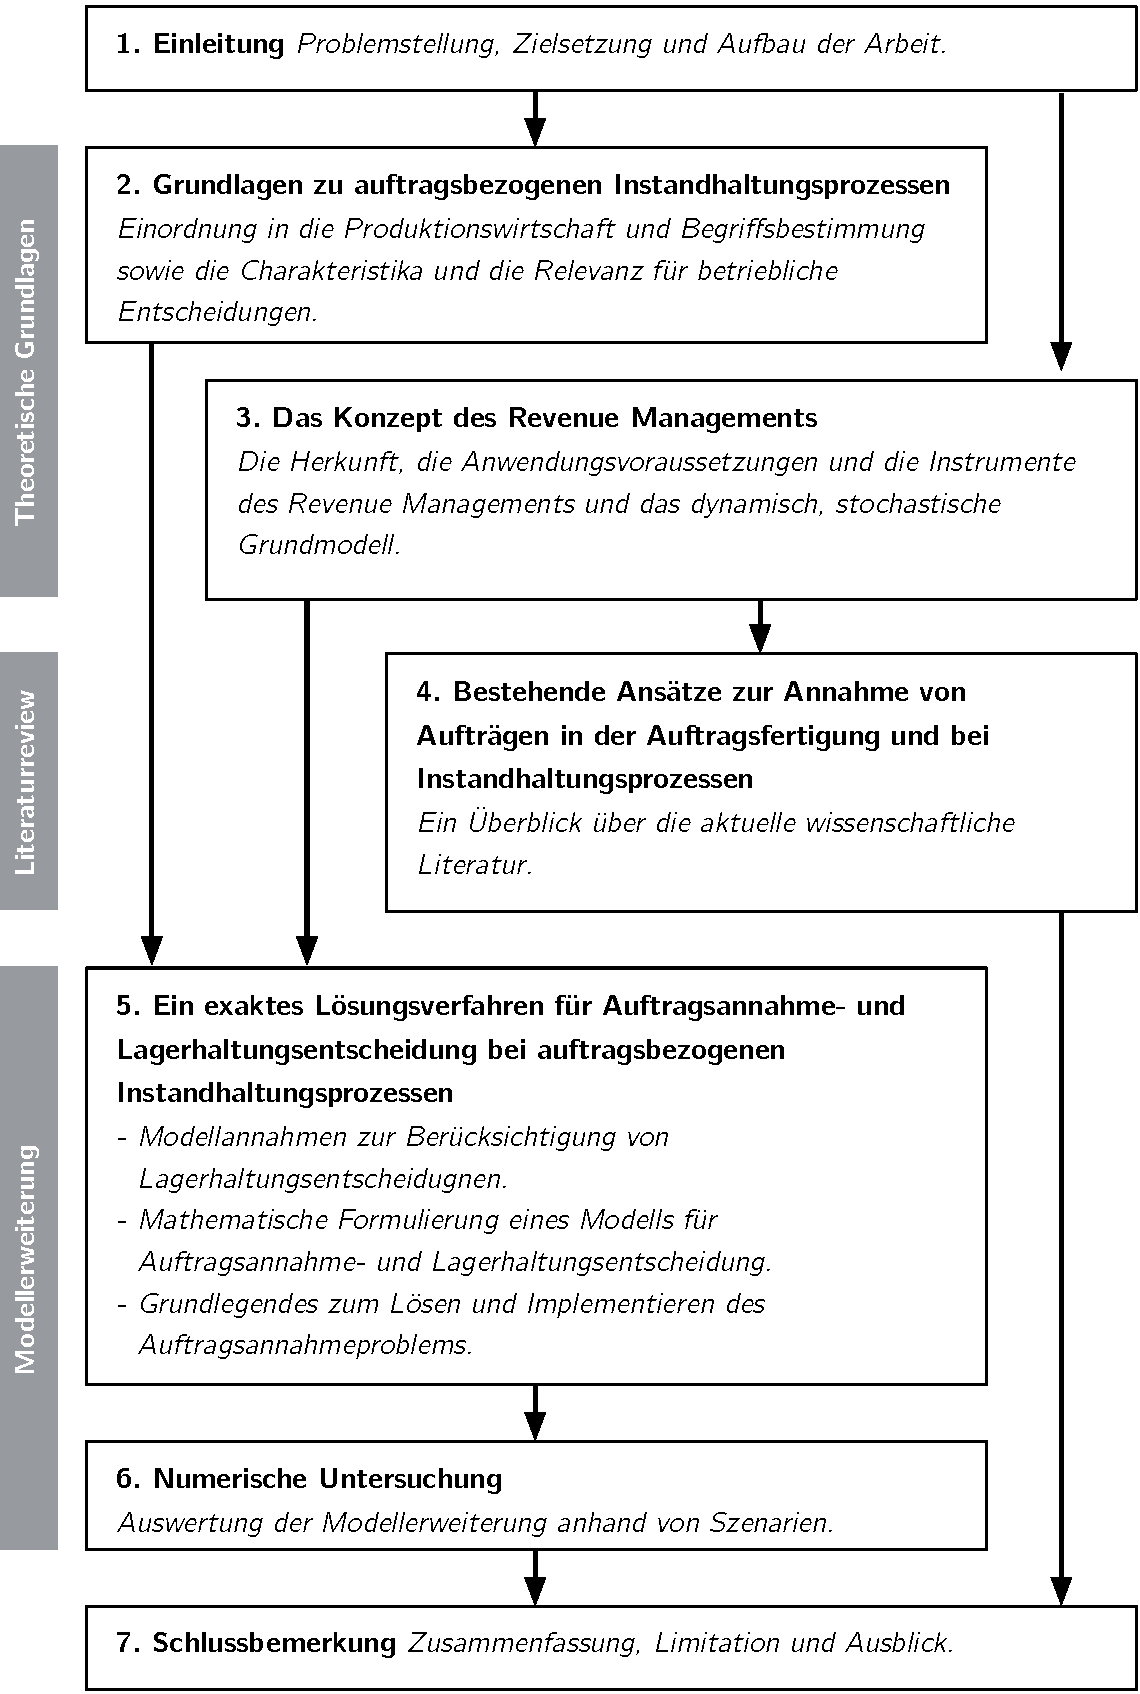
\includegraphics[width=140mm]{Bilder/Gliederung.pdf}
    \caption{Grafische Darstellung der Gliederung der Arbeit}  \label{Gliederung}
  \end{center}
\end{figure}


Der Aufbau der Arbeit ist in der Grafik \ref{Gliederung} dargestellt. In Kapitel 2 wird vorerst der Begriff der auftragsbezogenen Instandhaltungsprozessen definiert und deren theoretische Grundlagen beschrieben. In diesem Kapitel wird der Begriff in die Produktionswirtschaft eingeordnet, sowie die Beschreibung der Charakteristika und der Relevanz für betriebliche Entscheidungen der auftragsbezogenen Instandhaltungsprozessen aufgeführt. Weiter werden im Kapitel 3 die theoretischen Grundlagen der Arbeit vervollständigt, indem das Konzept des Revenue Management bei der Annahme von Aufträgen vorgestellt wird. In diesem Kapitel wird auf die Herkunft des Konzepts eingegangen. Für das Konzept bestehen zusätzlich Anwendungsvoraussetzungen und Instrumente, die in dem Kapitel beschrieben sind. Des Weiteren wird für das Grundmodell des Revenue Managements die mathematische Modellformulierung dargestellt.

Im Anschluss wird in Kapitel 4 ein Literaturüberblick über bestehende Ansätze zur Annahme von Auftragsproduktion und Instandhaltungsprozessen aufgeführt. Es werden hier vier Ansätze näher betrachtet, die den Fokus auf eine heuristische Lösung des Auftragsannahmeproblems legen.

Das Kapitel 5 zeigt die quantitative Untersuchung der Erweiterung des Grundmodells mit der Entscheidung über eine Lagerhaltung auf. Zum einen wird die  mathematische Modellformulierung und zum anderen wird ein Pseudo-Algorithmus zum exakten Lösen der Problemstellung beschrieben. Weiter werden die Grundlagen zur Implementierung des Pseudo-Alorithmus genannt. Im letzten Teil des Kapitels wird auf die numerische Untersuchung eingegangen.

Im letzten Kapitel sind die Schlussbemerkungen dieser Arbeit dargestellt. Es handelt dabei um eine Zusammenfassung der Ergebnisse der vorliegenden Arbeit und um einen Ausblick für nachfolgende Forschung.
% !TEX encoding = UTF-8 Unicode
\chapter{Grundlagen zu auftragsbezogenen Instandhaltungsprozessen}
\markboth{2 Grundlegende Begriffe}{}
\setcounter{footnote}{4}  %um durchgehende Fußnotennummerierung zu haben, hier die Anzahl der bisherigen Fußnoten eintragen

\section{Einordnung in die Produktionswirtschaft und die Begriffsbestimmung}

Unter auftragsbezogenen Instandhaltungsprozessen (engl. maintenance-repair-and\-overhaul (MRO)) wird in dieser Arbeit als ein nachgelagerter Prozess einer erweiterten Leistungserstellung verstanden und ist ein Teilsystem eines Unternehmens, welches den gesamten Wertschöpfungsprozess verlängert. Es handelt sich nicht um die interne oder beauftragte Instandhaltung von u. a. technischen Systemen, sondern um eine Erweiterung des Produktionsprogramm eines Unternehmens. Im weiteren Verlauf dieser Arbeit wird daher von MRO-Prozessen gesprochen. Da es bei MRO-Prozessen um eine Produktion einer Leistung handelt, werden diese der betriebswirtschaftlichen Betrachtung der Produktionswirtschaft zugeordnet.

Bei dem Begriff der Produktionswirtschaft handelt sich um ein Teilgebiet der Betriebswirtschaftslehre.\footnote{Neben der Teilgebiete Finanzwirtschaft, Marketing, Unternehmensführung, Unternehmensrechnung etc., vgl. dazu \cite{Dyckhoff2010}, S. 3.} In der Produktionswirtschaft wird der Fokus auf die Produktion von Leistung gelegt. Bei diesem ökonomischen Konzept wird die Transformation von materiellen und nichtmateriellen Inputgütern (Produktionsfaktoren) hin zu gewünschten Outputgütern (Leistung des Unternehmens) betrachtet. Bei den im Laufe der Zeit erweiterten betriebswirtschaftlichen Produktionsfaktoren nach \cite[S. 71]{Gutenberg:1959aa} handelt es sich um die Elementarfaktoren Werkstoffe, Betriebsstoffe, Betriebsmittel und objektezogene humane Arbeitsleistung sowie um die dispositiven Faktoren Betriebsführung, Organisation und Planung.\footnote{????} Bei Outputgütern handelt es sich um Produkte in Form von Sach- oder Dienstleistungen die dem Markt und somit der potentiellen Nachfrage der Marktteilnehmer zur Verfügung gestellt werden.\footnote{Vgl. \cite{Schmidt:2012aa}, S. 1.} Die Transformation erfolgt durch bestimmte von Menschen veranlasste unternehmerischen Verfahrensweisen.\footnote{Vgl. \cite{tempelmeier1994produktion}, S. 6, echt?????} Beispielsweise kann hier die industrielle Fertigung von Verbrauchs- oder Gebrauchsgütern genannt werden.

Bei der Transformation der Inputgüter erfolgt eine qualitative, quantitative, räumliche oder zeitlichen Veränderung der Objekte.\footnote{Vgl. \cite{Dyckhoff2010}, S. 3.} Durch diese Veränderung kann seitens des Unternehmens eine Leistung auf dem Markt angeboten werden. Damit diese Leistung den Absatz bei potentiellen Konsumenten findet, muss die Leistung durch die Transformation eine Wertschöpfung erhalten. Der konzeptionelle Rahmen dieses Gedankens bildet die Wertschöpfungslehre (engl. suppy chain management (SCM)).\footnote{Vgl. \cite{???}, S. ??.} Danach sollte das Ziel eines jeden Unternehmens das Betreiben von Wertschöpfung sein.\footnote{Vgl. \cite{???}, S. ??.} In der klassischen Auffassung der Wertschöpfungslehre durchläuft die Leistungserstellung alle (Teil-)Systeme des Unternehmens.\footnote{???} Abbildung \ref{Prozess} zeigt in Teil a. eine mögliche Abfolge der Systeme eines Unternehmens. Eine klassische Abfolge zur Leistungserstellung bzw. der Transformation von Inputgütern hin zu Outputgütern ist die Abfolge der Systeme Forschung/Entwicklung, Beschaffung, Produktion, Distribution sowie Verkauf. Damit ist die um die Wertschöpfung erhöhte Leistung auf dem Markt angekommen und das Unternehmen erzielt damit i. d. R. einen Ertrag (Revenue).

\begin{figure}[h!]
  \begin{center}
    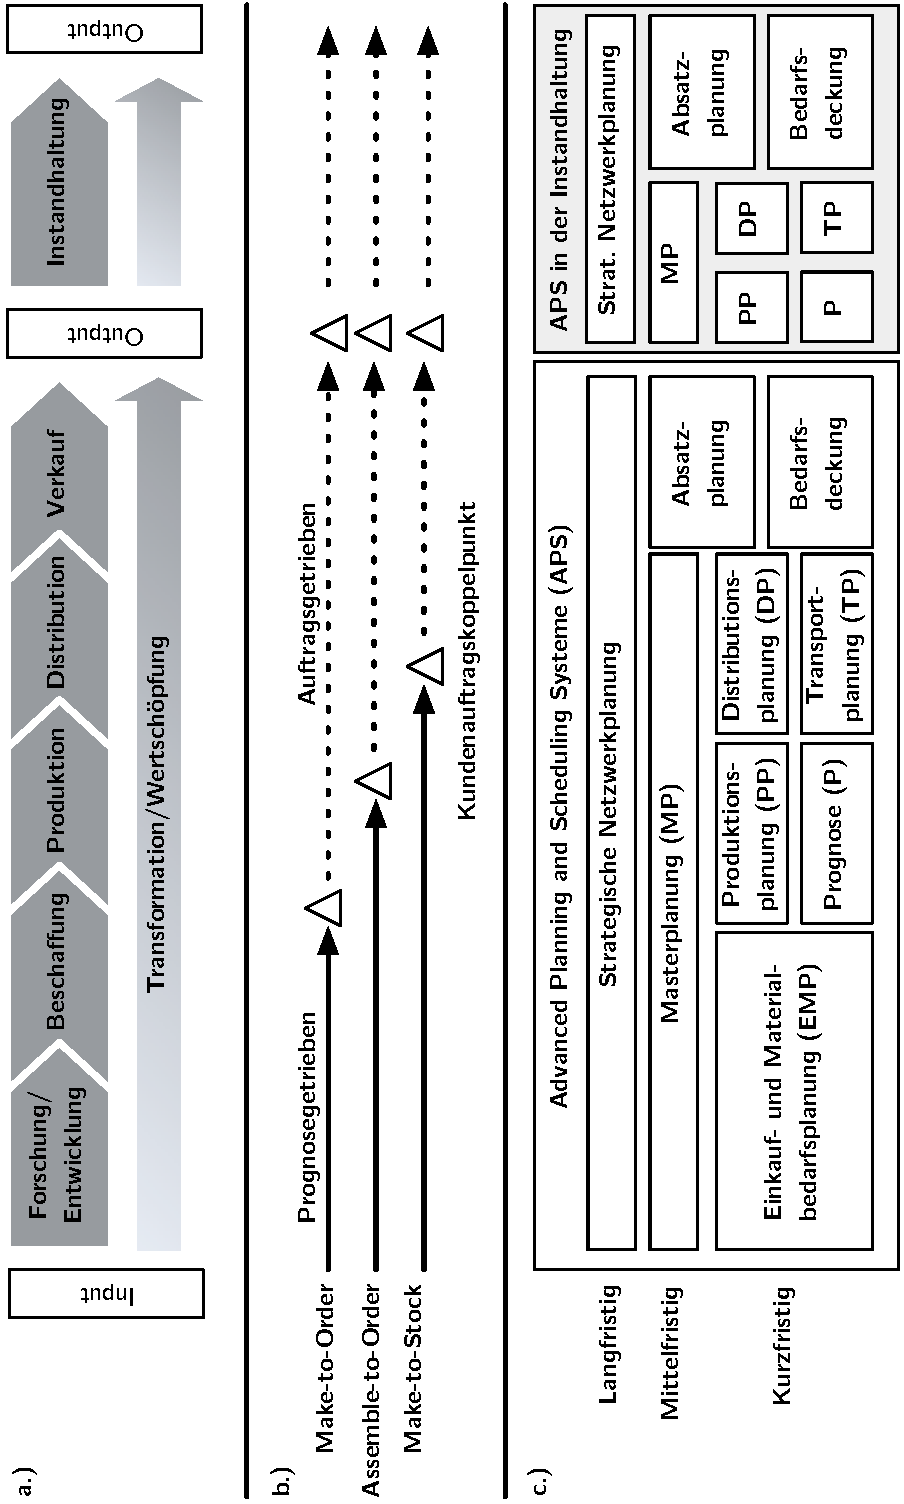
\includegraphics[width=100mm]{Bilder/prozess.pdf}
    \caption{Grafische Veranschaulichung eines Wertschöpfungsprozesses}  \label{Prozess}
    {\footnotesize \textbf{In Anlehnung an:} \cite{Bach:2012aa}, S. 4-5; \cite{quante2009management}, S. 21-22; \cite{meyr2015structure}, S. 100}
  \end{center}
\end{figure}

Sofern das Unternehmen eine \textbf{Instandhaltung} ihrer Leistungen anbieten kann, wird die Abfolge des Wertschöpfungsprozesses um dieses Unternehmenssystem erweitert. Für den gewerblichen Verkauf von Gütern an Privatkunden können gesetzliche Regelungen bestehen, womit ein Unternehmen gezwungen ist das Unternehmenssystem der Instandhaltung in den Wertschöpfungsprozess aufzunehmen.\footnote{Vgl. die Richtlinie 1999/44/EG des Europäischen Parlaments und des Rates vom 25. Mai 1999 zu bestimmten Aspekten des Verbrauchsgüterkaufs und der Garantien für Verbrauchsgüter.} Anderseits kann ein Unternehmen auch die Instandhaltung seiner eigenen Güter als eigenständige Leistung anbieten und damit den Gesamtertrag des Unternehmens erhöhen (MRO-Prozess). Dieses wird oft von Unternehmen angeboten, die ihren Umsatz mit komplexen Produkten erzielen. Komplexe Produkte zeichnen sich durch ihre hohe Anzahl an hochtechnologischen Komponenten aus, die erst durch den vollständigen und meist kostenintensiven Zusammenschluss eine individuelle Bedürfnisbefriedigung des Nachfragers ermöglichen.\footnote{Vgl. \cite{komplexe2009Schmidt}, S. 97} In dieser Arbeit werden solche komplexen Produkte betrachtet, die aus einer Vielzahl von Komponenten (Ressourcen) bestehen.

\citeauthor{helbing2010instandhaltung} versteht unter Instandhaltung die \glqq Gesamtheit der technischen und organisatorischen Mittel, Vorgänge und Maßnahmen zur Erhaltung, Verbesserung und Wiederherstellung des Funktions-, Leistungs- und Güteniveaus von materiellen Objekten während ihrer Wirkungs- und Lebenszeit durch Wartung, Inspektion und Instandsetzung.\grqq\footnote{Vgl. \citeauthor{helbing2010instandhaltung}, S. 984} In dieser Arbeit ist mit dem Begriff der MRO-Prozesse gemeint, dass für die betrachteten komplexen Produkte ein spezifischer Ausführungsmodus für die Anfragen verwendet wird, der eine erneute Integration von produkt-spezifischen Ressourcen vorsieht, damit die Funktionsfähigkeit des Produkts (Leistung) wiederhergestellt ist. Damit lässt sich das Verständnis des Begriffs als Leistung eines Unternehmens und als Unternehmenssystem ableiten, welches die Verlängerung und zugleich als Erweiterung des Wertschöpfungsprozesses versteht.

\section{Charakteristika}

Nach der DIN 310511 wird Instandhaltung insofern ausgeführt, wenn die Funktionsfähigkeit Betrachtungseinheit sichergestellt werden muss, damit der ursprüngliche Wert erhalten bleibt.\footnote{Vgl. \cite{Strunz:2012aa}, S. 1.} Betrachtungseinheit können ganze Anlagen und Maschinen sein oder nur einzelne Komponenten.\footnote{Vgl. \cite{schenk2010techSys}, S. 23.}

Erläuterung nach DIN 31051:\footnote{Unbedingt nachlegen!!!!}
\begin{itemize}
\item Instandhaltung ist die Kombination aller technischen und administrativen Maßnahmen des Managements während des Lebenszyklus einer Betrachtungseinheit zur Erhaltung des funktionsfähigen Zustandes oder der Rückführung in diesen, so dass sie die geforderte Funktion erfüllen kann.
\item Als Betrachtungseinheit (BE) wird jedes Bauelement, Gerät, Teilsystem, jede Funktionseinheit, jedes Betriebsmittel oder System, das für sich allein betrachtet werden kann, definiert.
\end{itemize}

Nach der DIN 31051 werden Einheiten betrachtet, die eine Wartung, Inspektion, Instandsetzung oder Verbesserung bedürfen. Bei einer Wartung handelt es sich um Maßnahmen zur Verzögerung der Abnutzung. Die Inspektion umfasst alle Maßnahmen der Begutachtung sowie der Beurteilung des Ist-Zustandes einer Betrachtungseinheit und die Instandsetzung beinhaltet die Maßnahmen zur Wiederherstellung des Sollzustands. Mit der Verbesserung sind Maßnahmen gemeint, die den Soll-Zustand der Betrachtungseinheit erweitern, damit mögliche Defekte verhindert werden.

Instandhaltungsprozesse lassen sich weiter nach Ausführungszeitpunkte und des Ausführungsorte der Maßnahmen unterscheiden.\footnote{Vgl. \cite{schenk2010techSys}, S. 24-26; \cite{hinsch2010instandhaltung}, S. 190-191} Diese Unterscheidung spielt bei der Betrachtung von MRO-Prozessen eine untergeordnete Rolle. 

Da der Absatz zeitlich vor der Produktion der Leistung stattfindet, handelt es sich bei dem hier betrachteten MRO-Prozessen um eine Auftragsfertigung.\footnote{Vgl. \cite{hax1956industriebetrieb}, S. 247; \cite{Gutenberg1965dispos}, S. 164-165} In der Literatur wird für die Auftragsfertigung oft der englischen Begriff \textit{Make-to-Order (MTO)} verwendet. Abzugrenzen ist der Begriff von der Lagerfertigung (engl. Make-to-Stock (MTS)) und der kundenindividuellen Fertigung mit standardisierten Komponenten (engl. Assemble-to-Order (ATO)). 
Dies kann zum einen anhand des Kundenauftragskoppelpunkt und zum anderen anhand der Planungsgrundlage der Leistungserstellung getätigt werden. Der Kundenauftragskoppelpunkt zeigt den erstmaligen Kundenkontakt bzw. Auftragseingang auf. Mit Eingang des Kundenauftrags wechselt die Planungsgrundlage der Leistungserstellung von prognosegetriebener hin zu auftragsgetriebener Planung. Die prognosegetriebenen Planungsgrundlage für die Fertigung ist mit einem Prognosefehler für die Wiederauffüllung der Ressourcen behaftet, was der analytischen Betrachtung des Kundenauftragskoppelpunkts zur Bestimmung der notwendigen Ressourcenkapazität und der weiteren Auftragseingänge weiteres Gewicht verleiht.\footnote{Vgl. \cite{quante2009management}, S. 21} 

Bei einer MTO trifft vor der eigentlichen Produktion der Leistung der Kundenauftrag ein. Damit sind die Forschungs/Entwicklung der Leistung und die Beschaffung der Komponenten bzw. Ressourcen hauptsächlich prognosegetrieben. Alle weiteren Teilsysteme des Unternehmens können sich speziell an den Forderungen des Auftrags richten. Ähnliche Rahmenbedingung besitzt eine ATO, die den Kundenauftragskoppelpunkt innerhalb des Produktionsablaufs hat. Da nur ein gewissen Umfang der Komponenten an auftragsspezifischen Eigenschaften angepasst wird, sind die Grundkomponenten der Produkte abhängig der Prognosemethoden des Unternehmens. Bei MTS erfolgt der Auftragseingang erst nach der Produktion, womit diese Fertigungsart den höchsten Anteil des Einsatzes von Prognosemethoden aufweist.\footnote{Vgl. \cite{fleischmeyr2004codp}, S. 300-303; \cite{quante2009management}, S. 21-22} Abbildung \ref{Prozess} zeigt im Teil b. die Unterschiede der Fertigungsarten im Verlauf des Wertschöpfungsprozesses. 

Da bei MRO-Prozessen erst mit Auftragseingang die erforderlichen Produktionsschritte und der Ressourcenbedarf bekannt sind, werden diese mit MTO-Prozessen gleichgesetzt. Zur Erfüllung möglichst vieler Aufträge muss eine möglichst gute Prognose der benötigen Ressourcen vorliegen, damit kurze Liefer- und Durchlaufzeiten gewährleistet bleiben.\footnote{Vgl. \cite{thaler2001supply}, S. 68.} Sofern die Prognose fehlerhaft ist und ein zu geringer Bestand an Ressourcen vorhanden ist, konkurrieren die unterschiedlich eintreffenden Anfragen nach MRO-Prozessen des Unternehmens bzgl. der Ressourcen untereinander. Sofern ein zu hoher Ressourcenbestand vorhanden ist, stellt sich die Frage über den besten Mix der unterschiedlichen Aufträge, damit die Ressourcenkapazität optimal genutzt wird und dementsprechend der Ertrag maximiert wird. Im nächsten Abschnitt wird dieser Frage in Bezug von Produktionsplanungssystemen und der betrieblichen Entscheidungsfindung weiter nachgegangen.

%Zur Produktionswirtschaft zählt die Planung und Steuerung des Produktionsprogramms und der Produktionsprozesse....


\section{Relevanz für betriebliche Entscheidungen}



% !TEX encoding = UTF-8 Unicode
\chapter{Das Konzept des Revenue Managements bei der Annahme von Aufträgen}
\markboth{2 Revenue Management in der Auftragsannahme}{}
\setcounter{footnote}{4}  %um durchgehende Fußnotennummerierung zu haben, hier die Anzahl der bisherigen Fußnoten eintragen


\section{Das Revenue Managements bei der Auftragsannahme}
Zur Entscheidungsunterstützung bei der Annahme von Kundenaufträgen wird in der aktuellen Forschung vermehrt auf das Konzept des Revenue Managements zurückgegriffen.\footnote{Vgl. \cite{klein2001revenue}, S. 246.} Da eine kurzfristige Anpassung der mittelfristig bereitgestellten Kapazitäten einer Dienstleistungsproduktion an eine unsichere und schwankende Nachfrage nicht möglich ist, wird mit dem Konzept eine effizientere Auslastung der bestehenden Kapazitäten ermöglicht.\footnote{Vgl. \cite{ing2005revenue}, S. 124.}

Der Begriff \textit{Revenue Management} wird im deutschsprachigen Raum meist mit \textit{Ertrags}\-\textit{management} oder \textit{Erlösmanagement} übersetzt.\footnote{Vgl. z. B. \cite{zehle1991yield}, S. 486} Yield Management wird als Synonym benutzt.\footnote{Vgl. z. B. \cite{kolisch2006revenue}, S. 319} Dabei greift der Begriff \textit{Yield} zu kurz, da damit in der Luftverkehrsbranche der Erlös je Passagier und geflogener Meile bezeichnet wird.\footnote{Vgl. z. B. \cite{weatherford1998tutorial}, S. 69} Der Term \textit{Revenue Management} hat sich jedoch gegenüber Yield Management durchgesetzt, da der Yield (Durchschnittsertrag) sich theoretisch durch nur einen Passagier maximieren lässt und somit die Maximierung als Zielsetzung nicht sinnvoll ist.\footnote{Vgl. \cite{Klein:2008aa}, S. 6; \cite{ing2005revenue}, S. 124-125.} Erste Ansätze des RM sind in der Praxis entwickelt. Durch die Deregulierung des amerikanischen Luftverkehrsmarktes im Jahr 1978 mussten die traditionellen Fluggesellschaften ihre Wettbewerbsfähigkeit gegenüber Billiganbietern erhöhen und entwickelten das frühe RM.\footnote{Vgl. \cite{Petrick:2009aa}, S. 1-3}

\cite{kimms2005revenue} versuchen durch eine umfangreiche Diskussion einige Erklärungsansätze aufzuzeigen (Warum? Wovon?). Zum einen hat das RM vor allem aus dem älteren, englischsprachigen Bereich einen engen Bezug zu konkreten Anwendungsgebieten. Sie zeigen auf, dass viele Autoren versuchen das komplexe Konzept des Revenue Managements in einer kurzen Erklärung zu überführen. Dieses läuft letztlich darauf hinaus, dass diese Autoren einige situative Merkmale und Instrumente des Managements vermischen, gleichzeitig aber versuchen, die Zielsetzung festzulegen und das Anwendungsgebiet auf bestimmte Branchen zu beschränken. %\cite{kimms2005revenue} weisen darauf hin, dass eine differenzierte Betrachtung des Konzepts notwenig ist: Einerseits im Hinblick auf die Anwendungsvoraussetzungen und andererseits im Hinblick auf die Instrumente des Revenue Managements, damit verdeutlicht dargestellt wird, in welchen Branchen das RM Potentiale liefert. In den nachfolgenden zwei Kapiteln wird dieser Empfehlung gefolgt.

Weiter wird in der Literatur der Begriff des RM unterschiedlich definiert. \cite{friege1996yield} bezeichnet das RM als \textit{Preis-Mengen-Steuerung}, \cite{daudel1992yield} als \textit{Preis-Kapazitäts-Steuerung} und \cite{talluri2004theory} verstehen es als das gesamtes \textit{Management der Nachfrage}. Die beiden ersteren Definitionen können als Synonym für eines der Instrumente des RM stehen und daher finden diese für das gesamte Konzept keine weitere Verwendung.\footnote{Vgl. z. B. \cite{Petrick:2009aa}} Nachfolgend wird die Definition von \citeauthor{klein2001revenue} (2001, S. 248) aufgegriffen:

\begin{quote}
\glqq Revenue Management umfasst eine Reihe von quantitativen Methoden zur Entscheidung über Annahme oder Ablehnung unsicherer, zeitlich verteilt eintreffender Nachfrage unterschiedlicher Wertigkeit. Dabei wird das Ziel verfolgt, die in einem begrenzten Zeitraum verfügbare, unflexibel Kapazität möglichst effizient zu nutzen.\grqq
\end{quote}

\cite{Petrick:2009aa} definiert das RM als Ziel einer Unternehmung die Gesamterlöse zu maximieren, die sich aufgrund der speziellen Anwendungsgebiete ergeben. Damit definiert \cite{Petrick:2009aa} das RM als Zusammenfassung aller Interaktionen eines Unternehmens, die mit dem Markt, also der Absatz- oder Nachfrageseite, zusammenhängen. Im Kern lassen sich drei wichtige Perspektiven für eine Definition des Revenue Managements nach \cite{Petrick:2009aa}, \cite{stuhlmann2000kapazitatsgestaltung},  \cite{corsten1999yield} übernehmen:
\begin{enumerate}
	\item Ziel ist es die Gesamterlöse unter möglichst optimaler Auslastung der vorhandenen Kapazitäten zu maximieren.
	\item Durch eine aktive Preispolitik wird das reine Kapazitäts- oder Auslastungsmanagement unterstützt.
	\item Für die erfolgreiche Implementierung des Revenue Managements ist eine umfangreiche Informationsbasis notwendig. Es muss u. a. eine möglichst gute Prognose über die zukünftige Nachfrage und Preisbereitschaft der Kunden vorhanden sein.
\end{enumerate}

\cite{kimms2005revenue} weisen darauf hin, dass eine differenzierte Betrachtung des Konzepts notwenig ist: Einerseits im Hinblick auf die \textbf{Anwendungsvoraussetzungen} und andererseits im Hinblick auf die \textbf{Instrumente des Revenue Managements}, damit verdeutlicht dargestellt ist, in welchen Branchen das RM Potentiale liefert. Dabei sollten branchenspezifische Besonderheiten, neben den zahlreichen Ähnlichkeiten Berücksichtigung finden, sowie das begrenzte Kapazitätenkontingent, damit die Potentiale des RM zur Maximierung der Gesamterlöse in den Dienstleistungsbranchen erfolgen kann.\footnote{Vgl. z. B. \cite{Martens:2009aa}, S. 11-24} In dem nachfolgenden Kapitel wird dieser Empfehlung gefolgt und die Anwendungsvoraussetzungen sowie Instrumente des RM vorgestellt.

\section{Anwendungsvoraussetzungen und Instrumente des Revenue Managements}

\cite{Petrick:2009aa} weist da\-rauf hin, dass anhand von speziellen Anwendungsvoraussetzungen geprüft wird, ob das RM für die jeweilige Situation des Unternehmens (oder die gesamte Branche) zur Maximierung des Gesamterlöses beiträgt. \cite{kimes1989yield} definiert die in der Literatur häufigsten Anwendungsvoraussetzungen:\footnote{Vgl. u. a. \cite{friege1996yield}, S. 616-622, und \cite{weatherford1992taxonomy}, 831-832.}
\begin{itemize}
	\item \glqq weitgehend fixe\grqq\;Kapazitäten
	\item \glqq Verderblichkeit\grqq\;bzw. \glqq Nichtlagerfähigkeit\grqq\;der Kapazitäten und der Leistung
	\item Möglichkeit zur Vorausbuchung von Leistungen
	\item stochastisch, schwankende Nachfrage
	\item hohe Fixkosten für die Bereitstellung der gesamten Kapazitäten bei vergleichsweise geringen variablen Kosten für Produktion einer Leistungseinheit
	\item Möglichkeit zur Marktsegmentierung und im Ergebnis dessen zur segmentorientierten Preisdifferenzierung
\end{itemize}
\vspace{0.2cm}
Aufgrund der Anwendungsvoraussetzungen des RM kann das Konzept auch auf die Auftragsfertigung bzw. MRO-Prozesse übertragen werden.\footnote{Vgl. \cite{hintsches2010revenue}, S.176-178; \cite{kimes1989yield}, S. 349-351.} Bei der Auftragsfertigung wird ein bestimmter Buchungszeitraum betrachtet, in dem weitestgehend von fixen Kapazitäten der Ressourcen ausgegangen werden kann. Durch Ablauf des Buchungshorizonts verfällt die Kapazität, da es sich hauptsächlich um erneuerbaren Kapazitäten handelt (Arbeitskraft, Maschinenkapazität, usw.). Anders formuliert, werden die Ressourcen zur nächsten Leistungserstellung erneuert. Dabei beschreibt $t$ einen Zeitpunkt des Buchungshorizonts. Die Gesamtlänge des Buchungshorizonts entspricht $T$ und verläuft rückwärts bis zur Leistungserstellung des betrachteten Buchungshorizonts. Da der Buchungshorizont mit genau einer Leistungserstellung gekoppelt ist, können diese mit einem Parameter $i$ beschrieben werden. Mit der Leistungserstellung werden die verbuchten Kapazitäten aus dem Buchungshorizont durch die Auftragsproduktion beansprucht. Mit dem Start der Leistungserstellung erfolgt ebenfalls die Vorausbuchungszeit für die nachfolgende Leistungserstellung $i+1$. Bei der Leistungserstellung $i+1$ sind die Kapazitäten der Ressourcen regeneriert.

\begin{figure}[h!]
  \begin{center}
    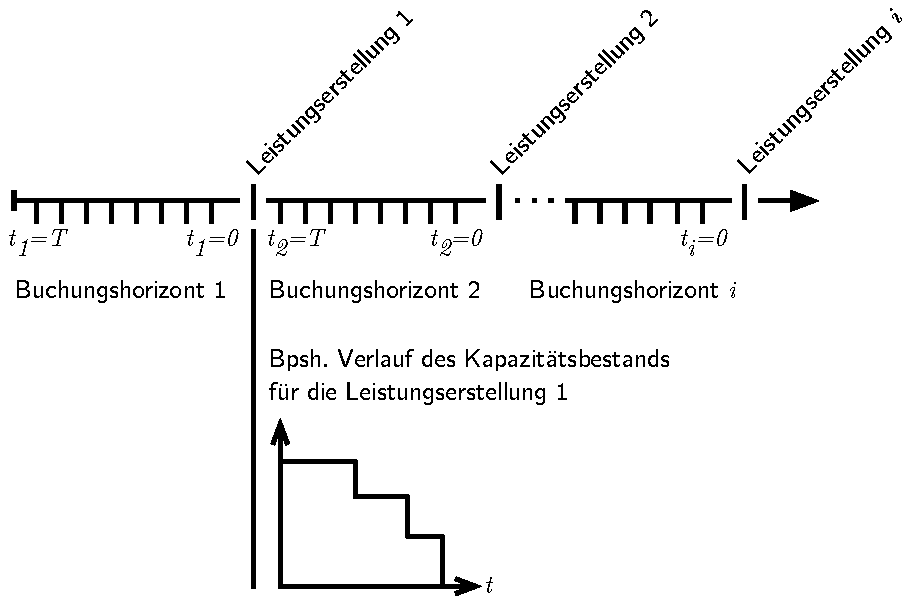
\includegraphics[width=140mm]{Bilder/Kapaverbrauch.pdf}
    \caption{Grafische Darstellung des Buchungshorizonts bei der Auftragsfertigung}  \label{B0}
    {\footnotesize \textbf{In Anlehnung an:} ???.} 
  \end{center}
\end{figure}


??? \cite{Klein:2008aa} setzen sich mit den Anwendungsvoraussetzungen von mehreren Autoren auseinander. Sie konnten Gemeinsamkeiten innerhalb der Definitionen der Autoren finden, aber zeigten auch die Unterschiede und die Kritiken auf. In ihrer Arbeit übernehmen sie die Anwendungsvoraussetzung von \cite{corsten1998yield}: "Marktseitige Anpassungserfordernis steht unternehmesseitigig unzureichendes Flexibilitätspotential hinsichtlich der Kapazität -- bezogen auf Mittel- oder Zeitaufwand -- gegenüber". Zugleich weisen sie jedoch darauf hin, dass zum Verständnis eines komplexen und interdisziplinären Ansatzes auch die Definitionen anderer Autoren im Hinblick auf das Verständnis der Anwendungsvoraussetzungen beitragen. ???

Auf Grundlage der von \cite{friege1996yield} beschriebenen Anwendungsvoraussetzungen hat \cite{Petrick:2009aa} drei Instrumente des RM bestimmt. Die Instrumente benötigen als Grundlage \textit{Daten der Prognose}, damit sie zur Anwendung kommen.\footnote{Die Prognose zählt laut \cite{Petrick:2009aa} nicht als eigenständiges Instrument des RM.} Zu den Instrumenten zählen die \textbf{segmentorientierte Preisdifferenzierung}, die \textbf{Kapazitäten\-steuerung} und die \textbf{Über\-buchungssteuerung}. Es lassen sich unterschiedliche Ab\-hängigkeit\-en der Instrumente untereinander ermitteln.\footnote{Als Beispiel baut die Kapazitätensteu\-erung auf den Ergebnissen der Preisdifferenzierung auf und die Überbuchungssteuerung kann selten ohne Kapazitätensteuerung gelöst werden.}

Erklärung segmentorientierte Preisdifferenzierung, Kapazitätssteuerung, Überbuchungssteuerung?

\section{Mathematische Modellformulierung des Revenue Managements}
Im Folgenden wird das dynamisch, stochastische Grundmodell des RM nach \citeauthor{talluri2004revenue} (2004, S. 18-19) beschrieben. Ein Dienstleistungsnetzwerk eines Anbieters benötigt jeweils zur Erstellung der Dienstleistungen ein bestimmtes Kontingent an Ressourcen aus einer Menge an Ressourcen $\mathcal{H} = \{1,...,l \}$. Der Index $h$ beschreibt dabei eine jeweilige Ressource und der Index $l$ die gesamte Anzahl an möglichen Ressourcen. Die jeweilige Kapazität einer Ressource $h \in \mathcal{H}$ ist durch den Parameter $c_{h}$ beschrieben und die gesamten Kapazitäten der Ressourcen ist als Vektor $\textbf{c}=(c_{1},...,c_{h},...,c_{l})$ formuliert. Eine Anfrage nach einem Produkt (Dienstleistung) in dem Netzwerk ist durch den Parameter $j$ aus der Menge an möglichen Produktanfragen $\mathcal{J} = \{1,...,n \}$ %für die Menge der Ressourcen $\mathcal{H}$
beschrieben. Die gesamte Anzahl an Produktanfragen ist durch den Parameter $n$ definiert. Sobald eine Produktanfrage $j\in \mathcal{J}$ akzeptiert und somit abgesetzt ist, fällt für den Absatz der Ertrag $r_{j}$ an. Der jeweilige Verbrauch einer Ressource $h$ durch Annahme einer Anfrage nach einem Produkt $j$ ist anhand des Parameters $a_{hj}$ beschrieben. Durch Vektorschreibweise kann der Ressourcenverbrauch für eine Anfrage nach einem Produkt $j$ als Vektor $\textbf{a}_{j}=(a_{1j},...,a_{hj},...,a_{lj})$ formuliert werden. Der Buchungshorizont entspricht $T$ Perioden und kann jeweils in einzelne Perioden $t=1,...,T$ aufgeteilt werden. Dabei muss Beachtung finden, dass der Buchungshorizont $T$ gegenläufig verläuft. Die Wahrscheinlichkeit der Nachfrage eines Produkts $j$ in der Periode $t$ entspricht $p_{j}(t)$ und die Wahrscheinlichkeit, dass keine Nachfrage in der Periode $t$ eintrifft, entspricht $p_{0}(t)$. Es gilt $\sum_{j\in \mathcal{J}}p_{j}(t)+p_{0}(t)=1$ und somit kann $p_{0}(t)$ durch den Term $p_{0}(t)=1-\sum_{j\in \mathcal{J}}p_{j}(t)$ für die Periode $t$ ermittelt werden.\footnote{Vgl. \citeauthor{talluri2004revenue}, S. 18} Die noch erwartete Nachfrage $D_{jt}$ für ein bestimmtes Produkt $j$ für eine beliebige Periode $t$ lässt sich durch $\sum_{\tau=1}^{t}p_{j}(\tau)$ aggregieren. 


Mit den vorangegangenen Parametern kann der maximal erwartete Ertragswert $V(\textbf{c},t)$ für eine Periode $t$ bei einer noch vorhandenen Ressourcenkapazität $\textbf{c}$ als Bellman-Gleichung formuliert werden (\textbf{DP-op}):\footnote{???}
\begin{equation}\label{DP}
V(\textbf{c},t)=\sum_{j\in\mathcal{J}}p_{j}(t)\max[ V(\textbf{c},t-1),\; r_{j}+V(\textbf{c}-\textbf{a}_{j},t-1)]+p_{0}(t)V(\textbf{c},t-1)
\end{equation}


Es handelt sich hier um die Modellformulierung der Dynamischen Programmierung (DP) im Netzwerk RM. Das Konzept der DP wurde von \citeauthor{bellman1954theory} entwickelt und dient der Ermittlung der optimalen Politik in Bezug auf den aktuellen Zustand eines Systems.\footnote{Vgl. \cite{bellman1954theory}, S. 4-5} Dabei bildet jeder Erwartungswert $V(\textbf{c},t)$ mit der Ressourcenkapazität $\textbf{c}$ zum Zeitpunkt $t$ einen Systemzustand des Netzwerks ab. Eine derartige Formulierung eines Optimierungsproblems wird oft als sogenannte \textit{Bellman'sche Funktionsgleichug oder Bellman-Gleichung} bezeichnet.\footnote{???}

Die Gleichung weist die Grenzbedingungen
\begin{equation}\label{GB1}
V(\textbf{c},0)=0 \text{ wenn } \textbf{c}\ge0 \text{ sowie }
\end{equation}
\begin{equation}\label{GB2}
V(\textbf{c},t)=-\infty \text{ wenn } c_{j}<0 \;\forall j\in\mathcal{J}
\end{equation}
auf, da eine jeweilig verbleibende Kapazität nach Bereitstellung des Produkts wertlos und eine negative Ressourcenkapazität nicht möglich ist. 

Die Gleichung \eqref{DP} lässt sich umformen, indem die Entscheidungen über die Annahme und Ablehnung einer Produktanfrage separiert wird. Da $\sum_{j\in \mathcal{J}}p_{j}(t)+p_{0}(t)=1$ gilt, kann die Gleichung weiter vereinfacht werden:\footnote{Vgl. \cite{Spengler:2007aa}, S. 161.}
\begin{equation*}
V(\textbf{c},t)=\sum_{j\in\mathcal{J}}p_{j}(t) V(\textbf{c},t-1) + \sum_{j\in\mathcal{J}}p_{j}(t) \max[r_{j}-V(\textbf{c},t-1)+V(\textbf{c}-\textbf{a}_{j},t-1,0)]+p_{0}(t)V(\textbf{c},t-1)
\end{equation*}
\begin{equation}\label{DP2}
=V(\textbf{c},t-1) + \sum_{j\in\mathcal{J}}p_{j}(t) \max[r_{j}-V(\textbf{c},t-1)+V(\textbf{c}-\textbf{a}_{j},t-1),0]
\end{equation}

Eine eintreffende Anfrage nach einem Produkt $j$ ist demnach dann akzeptiert, wenn der Ertrag $r_{j}$ größer gleich der Differenz des Erwartungswertes des Ertrags unter der Prämisse der Annahme der Produktanfrage und des Erwartungswertes des Ertrag unter der Prämisse der Ablehnung der Produktanfrage ist:
\begin{equation}\label{r}
r_{j} \ge V(\textbf{c},t-1)-V(\textbf{c}-\textbf{a}_{j},t-1)
\end{equation}

Dabei kann der rechte Term \eqref{r} als Opportunitätskosten (OK) der Auftragsannahme angesehen werden:
\begin{equation}\label{OC}
OC_{j} = V(\textbf{c},t-1)-V(\textbf{c}-\textbf{a}_{j},t-1)
\end{equation}

Somit erfolgt die Akzeptanz einer Anfrage nach einem Produkt $j\in\mathcal{J}$ ausschließlich nur dann, sofern die OK des Ressourcenverbrauchs niedriger als der Ertrag ist. Der maximal mögliche Erwartungswert unter Beachtung des Kapazität $\textbf{c}$ zum Zeitpunkt $t$ ist damit der Erwartungswert unter der Prämisse der Ablehnung der Anfrage zum nächsten Zeitpunkt $t-1$ inkl. der Summe der Erträge abzgl. der OK durch Annahme der möglichen Anfragen über aller Produkte $j\in\mathcal{J}$ und lässt sich mathematisch wie folgt definieren:
\begin{equation}\label{DPoc}
V(\textbf{c},t)=V(\textbf{c},t-1) + \sum_{j\in\mathcal{J}}p_{j}(t) \max[r_{j}-OC_{j},0]
\end{equation}

Die optimale Politik des Netzwerks zum Zeitpunkt $t$ ist damit die Annahme der Anfrage nach Produkt $j$ mit dem höchsten Ertrag $r_{j}$ bzgl. der anfallenden $OC_{j}$:

\begin{equation}\label{OP}
OP_{\textbf{c}, t}:= \{ \; j\; | \max_{j\in\mathcal{J}} [r_{j}-OC_{j}] \} 
\end{equation}

Zur Veranschaulichung des Netzwerk RM wird ein Netzwerk mit zwei Produkten $j\in\mathcal{J}$ und zwei Ressourcen $h\in\mathcal{H}$ betrachtet. Die Ressource $h=1$ hat eine Kapazität von $c_{1}=2$ und die Ressource $h=2$ hat eine Kapazität von $c_{2}=1$. Zur Ausführung des Produkt $j=1$ wird die Ressource $h=1$ mit einer Einheit benötigt und zur Ausführung des Produkt $j=2$ wird wiederum eine Einheit der Ressource $h=2$ gebraucht. Damit gilt $a_{11}=1$ und $a_{22}=1$. Durch Annahme einer Anfrage nach Produkt $j=1$ wird der Ertrag $r_{1}=100$ und durch Annahme von Produkt $j=2$ eine Ertrag von Ertrag $r_{2}=200$ generiert. Der Buchungshorizont entspricht $T=4$. Die Wahrscheinlichkeiten des Eintreffens eine Anfrage nach Produkt $j=1$ über die Buchungsperioden $t\in T$ lässt sich als Vektor $p_{1}(t)=(0.5, 0.5, 0.5, 0.5)$ beschreiben. Analog lassen sich die Wahrscheinlichkeiten für das Eintreffen der Produktanfragen $j=2$ als Vektor $p_{2}(t)=(0.1, 0.1, 0.1, 0.1)$ definieren. Die Gegenwahrscheinlichkeiten, dass keine Anfragen eintreffen, lassen sich mit $p_{0}(t)=1-\sum_{j\in \mathcal{J}}p_{j}(t)$ berechnen und bilden den Vektor $p_{0}(t)=(0.4, 0.4, 0.4, 0.4)$. Durch Vereinfachung der Gleichung \eqref{DP} zur Gleichung \eqref{DP2} werden die Gegenwahrscheinlichkeiten $p_{0}(t)$ nicht mehr benötigt und im weiteren Verlauf der Arbeit nicht mehr berücksichtigt.

Die Parameter lassen sich damit abschließend wie folgt definieren:
\begin{center}
$j = \{1, 2\}, \; h = \{1, 2\}, \; r_{1} = 100, \; r_{2} = 200, \; \text{Startperiode } t=4$,
\end{center}
\[
    \textbf{c}=\begin{pmatrix} 2 \\ 1 \end{pmatrix}, \;
    \textbf{a}_1=\begin{pmatrix} 1 \\ 0 \end{pmatrix}, \;
     \textbf{a}_2=\begin{pmatrix} 0 \\ 1 \end{pmatrix}, \;
     p_{1}(t)=\begin{pmatrix} 0.5\\ 0.5\\ 0.5\\ 0.5  \end{pmatrix}, \;
     p_{2}(t)=\begin{pmatrix} 0.1\\ 0.1\\ 0.1\\ 0.1  \end{pmatrix}
  \]

Die mathematische Modellformulierung des stochastisch, dynamisches Programms aus Gleichung \eqref{DP2} lässt sich als Graph darstellen, da es sich um eine rekursive Form handelt. Der Erwartungswert $V(\textbf{c},t)$ ist abhängig vom Erwartungswert $V(\textbf{c},t-1)$ und vom Erwartungswert $V(\textbf{c}-\textbf{a}_{j},t-1)$. Der Erwartungswert $V(\textbf{c},t-1)$ ist wiederum abhängig vom Erwartungswert $V(\textbf{c},t-2)$ und vom Erwartungswert $V(\textbf{c}-\textbf{a}_{j},t-2)$, usw. Abbildung \ref{B0} zeigt die erste rekursive Folge für die Gleichung \eqref{DP2} als Graphen auf und im nachfolgenden wird auf die Notation eingegangen.
\begin{figure}[h!]
  \begin{center}
    \includegraphics[width=80mm]{Bilder/Beispiel0.pdf}
    \caption{Beispielhafte Darstellung einer rekursive Folge eines Netzwerk RM}  \label{B0}
  \end{center}
\end{figure}
Ein Knoten repräsentiert einen Systemzustand des Netzwerks mit den vorhandenen Kapazitäten $\textbf{c}$ zum Zeitpunkt $t$. Dabei wird als Benennung für den Knoten eine Zahlenfolge verwendet, bei dem die ersten Einträge die Ressourcenkapazität $\textbf{c}$ in Länge der Ressourcen $h$ entsprechen und der letzte Eintrag den Zeitpunkt $t$ aufzeigt. Bspw. zeigt der Startknoten die Zahlenfolge $[2\;1\;4]$, da das Netzwerk noch die volle Ressourcenkapazität $\textbf{c}=(2,1)$ aufweist und sich im Zeitpunkt $t=4$ befindet. Von diesem Systemzustand können jetzt nachfolgende Systemzustände abhängig der Produktanfragen erreicht werden. In diesem Netzwerk gibt es zwei Produkte $j$ und durch betrachten der Gleichung \eqref{DP2} wird klar, dass drei Optionen zum Erreichen des nachfolgenden Systemzustands zum Zeitpunkt $t-1=3$ möglich sind. Diese Optionen bilden die Kanten des Graphen. Es kann keine Anfrage nach einem Produkt $j$ eintreffend, dann wird der nachfolgende Systemzustand $[2\;1\;3]$ erreicht. Alternativ können Anfragen nach Produkt $j=1$ oder $j=2$ eintreffen und dementsprechend müssen die vorhanden Kapazitäten $\textbf{c}$ um den Ressourcenverbrauch $a_{11}=1$ bzw. $a_{22}=1$ reduziert werden. Daraus folgt, dass der Systemzustand $[1\;1\;3]$ bzw. $[2\;0\;3]$ im Netzwerk erreicht werden kann.

Aufbauen auf dieser rekursiven Logik wird ein kompletter Entscheidungsbaum (Gerichteter und gewichteter Multigraph) aufgebaut. Er zeigt alle möglichen Systemzustände des Netzwerks. Die Rekursion wird abgebrochen, sofern ein Systemzustand aufgrund der Grenzbedingungen aus den Gleichungen \eqref{GB1} oder \eqref{GB1} nicht möglich ist. Abbildung \ref{B1} zeigt den Entscheidungsbaum für das eingeführte Beispiel.
\begin{figure}[h!]
  \begin{center}
    \includegraphics[width=150mm]{Bilder/Beispiel1.pdf}
    \caption{Darstellung des Entscheidungsbaums des beispielhaften Netzwerk RM}  \label{B1}
  \end{center}
\end{figure}

Betrachten wird den Entscheidungsbaum mit den möglichen Systemzuständen aus der Abbildung \ref{B1} weiter, dann kann das Entscheidungsproblem der Auftragsannahme durch Rückwärtsinduktion gelöst werden.\footnote{Vgl. ???, S. ???.} Dafür wird im ersten Schritt die Grenzbedingung aus Gleichung \eqref{GB1} betrachtet. Alle Systemzustände zum Zeitpunkt $t=0$ nehmen den Erwartungswert $V(\textbf{c}, t=0)=0$ an. Mit dieser Bedingung lassen sich die zeitlich zuvorkommenden Systemzustände mit $t=1$ berechnen. Es wird die Gleichung \eqref{DP2} angewendet, wobei beachtet werden muss, dass nicht für alle Systemzustände mit $t=1$ alle Produktanfragen möglich sind. Dies folgt aus der Grenzbedingung aus Gleichung \eqref{GB2}. Zur Veranschaulichung wird der Erwartungswert des Systemzustands $[1\;0\;1]$ mittels der Gleichung \eqref{DP2} berechnet.
\begin{alignat*}{2}
V(1,0,1)=\;&V(1,0,0)+p_{1}(1)\max[r_{1}-V(1,0,0)+V(0,0,0),0]\\
&+p_{2}(1)\max[r_{2}-V(1,0,0)+V(0,-1,0),0]\\
=\;&0+0,5\cdot\max[100-0+0,0]+0,1\cdot\max[200-0+(-\infty),0]\\
=\;&0+0,5\cdot 100+0,1\cdot0\\
=\;&50\\
\end{alignat*}

Nach dieser Vorgehensweise der Rückwärtsinduktion erfolgt die Ermittlung alle Erwartungswerte der möglichen Systemzustände des Entscheidungsbaum. Tabelle \ref{Tab1} zeigt für den Entscheidungsbaum alle möglichen Systemzustände (Cap1, Cap2, Time) mit den Erwartungswerten (ExpValue) und den möglichen Nachfolgern (Successor).
\begin{table}
\begin{footnotesize}
    \caption{Ergebnistabelle für das beispielhafte Netzwerk RM} \label{Tab1}
    \vspace*{3mm}
\csvautotabular{data/beispiel1.csv}
      %{\footnotesize \textbf{In Anlehnung an:} \cite{gonsch2013using}, S. 113.} 
\end{footnotesize}
\end{table}

Zusätzlich zeigt die Tabelle die optimale Politik für jeden Systemzustand (Best Order, Best Successor, r[j]-OC[j]). Die optimale Politik $OP_{\textbf{c}, t}$ lässt sich anhand der Gleichung \eqref{OP} für jeden Systemzustand ermitteln. Für jede Kante im Entscheidungsbaum der Abbildung \ref{B1} kann damit der Ertrag abzgl. der OK hinterlegt werden ($r_{j}-OC_{j}$). Die optimale Politik $OP_{\textbf{c}, t}$ im betrachteten Systemzustand ist demnach die Kante bei der höchste Ertrag erzielt wird. Abbildung \ref{B1a} zeigt den Entscheidungsbaum mit den jeweiligen Erwartungswerten und der optimalen Politiken für jeden Systemzustand.
\begin{figure}[h!]
  \begin{center}
    \includegraphics[width=150mm]{Bilder/Beispiel1a.pdf}
    \caption{Darstellung des Entscheidungsbaums des beispielhaften Netzwerk RM (optimale Politiken)}  \label{B1a}
  \end{center}
\end{figure}

Mit diesem Ergebnis kann eine strategische Politik abgeleitet werden. Diese strategische Politik kann dem Unternehmen helfen seine Instrumente der Marktbearbeitung zu optimieren. In diesem kleinen Betrachtungsfeld $T=4$ sollte das Unternehmen zum Zeitpunkt $t=4$ versuchen seine Instrumente in der Form auszurichten, dass eine Anfrage nach Produkt $j=2$ eintrifft. Nachfolgend sollte das Unternehmen zum Zeitpunkt $t=3$ und $t=2$ den Absatz von Produkt $j=1$ vorantreiben. Damit wäre der optimale Pfad des Entscheidungsbaums gefunden ($[2\;1\;4] \rightarrow_{j=2} [2\;0\;3] \rightarrow_{j=1} [1\;0\;2] \rightarrow_{j=1} [0\;0\;1]\rightarrow_{j=0} [0\;0\;0]$). Mit dem optimalen Pfad ist ein Ertrag in Höhe von 400 GE generiert. Bei Abweichung des Pfads in der operativen Planung der Unternehmensaktivitäten, z. B. durch nicht eintreffen der Anfrage $j=2$ zum Zeitpunkt $t=4$, gibt das Modell einen anderen Pfad mithilfe der optimalen Politiken an. Bspw. trifft zum Zeitpunkt $t=4$ nur die Anfrage nach Produkt $j=1$ ein. Dann muss das Unternehmen seine Instrumente an den neuen Pfad anpassen ($[2\;1\;4] \rightarrow_{j=1} [1\;1\;3] \rightarrow_{j=2} [0\;1\;2] \rightarrow_{j=1} [0\;0\;1]\rightarrow_{j=0} [0\;0\;0]$). Damit ist trotz der Abweichung ein Gesamtertrag von 400 GE möglich.

Anhand des Beispiels wird klar, dass die Prognose über die Wahrscheinlichkeiten des Eintreffens einer Anfrage nach den Produkten $j\in\mathcal{J}$ die Erwartungswerte stark beeinflussen. Der potentielle Ertrag $r_{j}$ und die $OC_{j}$ beeinflussen maßgeblich die optimale Politik. Dies kann durch das Abwandeln der Parameter gezeigt werden:
\begin{center}
$j = \{1, 2\}, \; h = \{1\}, \; r_{1} = 100, \; r_{2} = 150, \; T=4$
\end{center}
\[
    c_{1}= 3, \;
    a_11=1, \;
     a_12=2, \;
     p_{1}(t)=\begin{pmatrix} 0.5\\ 0.5\\ 0.5\\ 0.5  \end{pmatrix}, \;
     p_{2}(t)=\begin{pmatrix} 0.1\\ 0.1\\ 0.1\\ 0.1  \end{pmatrix}
  \]
Bei dieser Definition der Parameter konkurrieren die Typen der Produktanfragen $j$ mit der einzigen Ressource $h$. Der nachfolgende Abbildung \ref{B2} zeigt den zugehörigen Entscheidungsbaum mit den Systemzuständen, den möglichen Entscheidungen und der grafischen Darstellung der optimalen Politik und die Tabelle \ref{Tab2} zeigt die berechneten Erwartungswerte sowie die optimale Politik anhand des um die OK reduzierten Ertrags für jeden Systemzustand.

\begin{figure}[h!]
  \begin{center}
    \includegraphics[width=150mm]{Bilder/Beispiel2.pdf}
    \caption{Darstellung des Entscheidungsbaums des Netzwerk RM mit konkurrierenden Anfragen}  \label{B2}
  \end{center}
\end{figure}

\begin{table}
\begin{footnotesize}
    \caption{Ergebnistabelle für das beispielhafte Netzwerk RM mit konkurrierenden Anfragen} \label{Tab2}
    \vspace*{3mm}
\csvautotabular{data/beispiel2.csv}
      %{\footnotesize \textbf{In Anlehnung an:} \cite{gonsch2013using}, S. 113.} 
\end{footnotesize}
\end{table}

Mit dem Beispiel wird klar, dass trotz des höheren Ertrags der Produktauftrags $j=2$ im Systemzustand $[3\,4]$ die optimale Politik die Annahme bzw. Vorausbuchung der Produktanfrage $j=1$ ist. Aufbauend auf dieser Entscheidung ist der optimale Pfad $[3\;4] \rightarrow_{j=1} [2\;3] \rightarrow_{j=1} [1\;2] \rightarrow_{j=1} [0\;1]\rightarrow_{j=0} [0\;0]$ und es wird ein Gesamtertrag von 300 GE generiert. Trifft zum Systemzustand $[3\,4]$ jedoch keine Anfrage ein ($j=0$), dann ist die optimale Politik im Systemzustand $[3\,3]$ die Annahme der Produktanfrage $j=2$. Dies resultiert aus der Tatsache, dass die OK dem potentiellen Ertrag entgegenwirkt. Durch diese Eigenschaft gelangt das System zum Zustand $[1\,2]$ mit einem Ertrag von 150 GE. In diesem System wäre über zwei Perioden noch die Annahme einer Anfrage $j=1$ möglich.

% !TEX encoding = UTF-8 Unicode
\chapter{Bestehende Ansätze zur Annahme von Aufträgen in der Auftragsfertigung und bei Instandhaltungsprozessen}\label{Review}
\markboth{4 Bestehende Ansätze}{}
\setcounter{footnote}{4}  %um durchgehende Fußnotennummerierung zu haben, hier die Anzahl der bisherigen Fußnoten eintragen

Das Konzept des Revenue Managements (RM) zur Annahme von Aufträgen bei Dienstleistungen findet bereits über mehrere Dekanen in der wissenschaftlichen Literatur Anwendung.\footnote{Vgl. Klein (2001), S. 246.} Neue Veröffentlichungen versuchen das Konzept auf die Problemstellung der Annahme von Anfragen der Auftragsfertigung bzw. Kundeneinzelfertigung zu übertragen. Wie in Kapitel \ref{Instandhaltung} dargelegt, kann der Instandhaltungsprozess eines Dienstleistungsunternehmens einer Auftragsfertigung gleichgesetzt werden. \cite{kimms2005revenue} geben einen Überblick über das traditionelle Konzept des RM über verschiedene Branchen. Dabei schreiben die Autoren, dass das Konzept des RM vermehrt Anwendung findet, damit Unternehmen eine Unterstützung in der Entscheidungsfindung erhalten, welche Aufträge zur Auftragsfertigung akzeptiert werden sollen.\footnote{Vgl. \cite{kimms2005revenue}, S. 1.} \cite{quante2009management} gibt einen Überblick über relevante Literatur des traditionellen RM. Tabelle \ref{Überblick} zeigt eine Anlehnung der Übersicht von \cite{quante2009management} mit den Publikationen zum traditionellen RM in der Fertigungsindustrie. Die Tabelle zeigt jeweils zur Publikation den Kundenauftragskoppelpunkt, die Anzahl der berücksichtigen Konsumerklassen und die Methode aufgeführt ist. Die Konsumerklassen resultieren aus der für das Konzepts des Revenue Management notwendigen Marktsegmentierung von Kunden bzw. Auftragstypen. Einige Konzepte und Modelle berücksichtigen daher explizit die Anzahl solcher Klassen.

\renewcommand{\arraystretch}{1.2}
\begin{table}[h!]
  \begin{center}
    \caption{Überblick über Publikationen des traditionellen Konzepts des Revenue Managements in der Fertigungsindustrie}  \label{Überblick}
    \vspace*{3mm}
    \begin{tabular}{llll}   %hier die Spaltenausrichtung, -breite, -begrenzung und -anzahl eintragen
     Autoren & KAKP  & \#Klassen & Methode  \\ \hline
     \cite{deBHarris1995299} &      ATO          &  2  &  K, M \\
      \cite{Kalyan:2002aa}      &      MTO/ATO/MTS          &  --  &  K \\
                \cite{rehkopf:2005aa}   &      MTO          &  mehrere &  K, M \\
                      \cite{rehkopf2007revenue}    &      MTO          &  --  &  K, M, L \\
                               \cite{Spengler:2007aa}   &    MTO            & mehrere & M  \\
                               \cite{Volling20121021} & MTO & -- & K, M \\
          \cite{kimms2005branchenverg} & MTO & -- & K \\
          \cite{guhlich2015revenue} & ATO & -- & M, L \\
          \cite{kolisch2006revenue} & MTO & -- & K \\
              \cite{DECI:DECI074}  &      MTO          &  mehrere  &  M \\
    % Kumar and Frederick            &      MTO/MTS          &  3  &  F \\
          \cite{kuhn2004revenue} & MTO & 2 & F \\
        \cite{Specht:2008aa} &        ATO    &  --  & K, F  \\
        \cite{quante2009revenue} & MTO & -- & L \\ 
        \cite{cheraghi2010revenue} & MTO/MTS & -- & L \\
        \cite{sucky2009revenue} & MTO & -- & M, F \\ \hline
    \end{tabular} \\[3mm]
    {\footnotesize \textbf{In Anlehnung an:} \cite{quante2009management}, S. 44.}\\
        {\footnotesize \textbf{Legende:} KAKP: Kundenauftragskoppelpunkt, F: Fallstudie, K: Konzeption, L: Literaturüberblick, M: Simulations-/Analysemodell. }   %footnotesize liefert Schrift in Größe 10pt
  \end{center}
\end{table}

\cite{deBHarris1995299} beziehen die RM-Komponenten der differenzierten Preispolitik und eine multiklassen Kapazitätsallokation in ihr Modell mit ein. Sie zeigen, dass sofern stochastische Nachfrage auf fixe und kurzfristige Kapazität trifft, dass es zu Lagerfehlbeständen bei Niedrig-Preis-Segmenten führt. Jedoch rechtfertigen diese Lagerfehlbestände eine Premiumpreisstrategie bei den Kundengruppen mit höherer Preisbereitschaft, was letztendlich zu Umsatzsteigerungen führt.\footnote{Vgl. \cite{deBHarris1995299}, S. 307-308.} \cite{Kalyan:2002aa} beschäftigt sich mit der Bestätigung der Anwendungsvoraussetzungen des RM für die Auftragsfertigung. Das vom Autor beschriebene Konzept sieht die Einführung eines minimalen Akzeptanzwert vor. Sofern dieser Wert bekannt ist, kann ein Unternehmen bei jedem Auftragseingang die Entscheidung treffen, welche Anfrage angenommen oder abgelehnt werden soll.

Der vom Autor \cite{Kalyan:2002aa} eingeführte minimalen Akzeptanzwert wird in der wissenschaftlichen Literatur im Kontext des Konzepts des Revenue Managements als sogenannten Bid-Preis bezeichnet. Bei dem Bid-Preis handelt es sich um einen variierenden Parameter in Abhängigkeit der Zeit (bzw. der Periode) und der verfügbaren Ressourcenkapazität des betrachteten Netzwerks. Er kann als statische Information der optimalen Lösung für die eindimensionalen Probleme angesehen werden. Die Ermittlung des Bid-Preises erfolgt bei den traditionelle Modellformulierungen des RM anhand des \textit{deterministische lineare Programm (DLP)} unter deterministisch eintreffenden Nachfragen.\footnote{Vgl. \cite{talluri2004revenue}, S. 107-108.} %Der Bid-Preis korrespondiert zur Entscheidungsvariable $x_{jm}$ des DLP, da er verbunden ist mit der Kapazität einer jeden Ressource $h$.\footnote{Vgl. \cite{gonsch2013using}, S. 98}
Er fungiert als Schwellenpreis für eine jede Ressource im Netzwerk und ist normalerweise beschrieben als geschätzte marginale Kosten aufgrund des nächsten sukzessiven Verbrauchs einer Einheit der Ressourcenkapazität.\footnote{Vgl. \cite{talluri2004theory}, S. 89.} Laut \cite{gonsch2013using} erfolgt der Ansatz erstmalig von \cite{talluri2001airline} in Verbindung der Optimierung von Passagierrouten. Das Verfahren des Bid-Preises ist ein einfacher Weg, die Kapazitäten der Ressourcen in einem Netzwerk eines Anbieters zu kontrollieren.\footnote{Vgl. \cite{talluri2004theory}, S. 86-87\label{RMH}.} Viele Konzepte der neueren Veröffentlichungen im Bereich des Netzwerk RM sehen die Verwendung des Bid-Preise vor.\footnote{Vgl. \cite{petrick2010dynamic}, S. 2028; \cite{gonsch2013using}, S. 98-100.}

%Der Bid-Preis stellt das dynamische Minimum dar, zu dem eine Unter- nehmung bereit ist eine Leistung zu erstellen. Vor allem für Probleme vernetzter Leis- tungserstellung ist die Methode des Bid-Preises besonders geeignet. Tscheulin/Lindenmeier (2003), S. 639.

\cite{rehkopf:2005aa} zeigen durch das Lösen eines linearen Modells die Kapazitätsallokation für die Problemformulierung des Netzwerk-RM im Fall von MTO-Prozessen. Die Autoren fokussieren sich dabei auf die Branche der Eisen- sowie Stahlindustrie und veröffentlichen zwei Publikationen mit ihren Forschungsergebnissen. Dabei findet der im vorherigen Absatz definierte Bid-Preis Anwendung. 

\cite{rehkopf2007revenue} verfasste nach Veröffentlichung der ersten Publikation eine Schrift zu einem umfangreichen RM-Konzept zur Auftragsannahme bei kundenindividueller Produktion. Auch hier wird als Beispiel der Anwendungsfall in der Branche der Einsen und Stahl erzeugenden Industrie untersucht. Es werden zwei Fallstudien betratet, die zum einen die taktisch-operative Allokation der Kapazität und zum anderen die operative Annahmeentscheidung beinhaltet. Bei der Entwicklung einer geeigneten RM-Methodik in der Stahl erzeugenden Industrie kommt zum Tragen, dass in dieser Branche eine strikt divergente Produktionsstruktur vorliegt und dadurch die Auftragsfertigung in einstufige Leistungserstellung zerlegt werden kann.\footnote{Vgl. \cite{rehkopf2007revenue}, S. 113.} Dabei konnte die Fallstudie zeigen, dass bei der taktisch-operativen Allokation der Kapazität das vorgestellte Verfahren des RM mit einem FCFS-Verfahren eine ausgesprochene Dominanz gegenüber eines deterministischen Ansatzes mit FCFS-Verfahren aufweist.\footnote{Vgl. \cite{rehkopf2007revenue}, S. 127-134.} Für die operative Entscheidungsunterstützung formuliert der Autor ein Netzwerk-RM-Modell, welches durch ein spezielles Verfahren die Restkapazität bestimmt. Das Verfahren berechnet die Restkapazität nach einem real-time Ansatz für den zusicherbaren Bestand\footnote{Vgl. den Ansatz \glqq Available-to-promise\grqq.} aus der kapazitierten Hauptproduktionsprogrammplanung und den bereits eingeplanten Aufträgen des Netzwerks.\footnote{Vgl. \cite{rehkopf2007revenue}, S. 140; \cite{Spengler:2007aa}, S. 160.} Ebenso wird hier der Ansatz des Bid-Preises eingesetzt, welcher durch ein duales lineares Optimierungsmodell ermittelt wird.\footnote{Vgl. \cite{rehkopf2007revenue}, S. 144.} Dabei konnte er in der Fallstudie das Potential der Anwendung eines Bid-Preises und für den angewandte Ansatz zur Ermittlung der Restkapazität feststellen.\footnote{Vgl. \cite{rehkopf2007revenue}, S. 177.} Die Ergebnisse aus dieser Monografie fließen in die zweite Veröffentlichung von \cite{Spengler:2007aa}. In dieser Arbeit wird in einer Fallstudie ebenfalls gezeigt, dass durch eine Bid-Preis-Strategie der Gesamtdeckungsbeitrag verbessert wird.\footnote{Vgl. \cite{Spengler:2007aa}, S. 157–171.} Dabei werden in der Publikation die Bid-Preise jeweils mit einer linearen Modellformulierung sowie einer multi-dimensionalen Knaksack-Modell\-for\-mu\-lier\-ung berechnet und verglichen. Dabei wird deutlich, dass beide Verfahren den Deckungsbeitrag ähnlich verbessern, wobei sich das Lösen anhand der Knaksack-Modell\-for\-mu\-lier\-ung als robuster darstellt.\footnote{Vgl. \cite{Spengler:2007aa}, S. 168-169.} In der Arbeit zeigten die Autoren, dass durch Anwenden der Heuristik sich der Gesamterlös im Vergleich zu einer einfachen Reihenfolgeannahme\footnote{\glqq First come, first served\grqq.} um 5,3\% erhöhen lässt.\footnote{Vgl. \cite{Spengler:2007aa}, S. 170.}

\cite{Volling20121021} beschäftigen sich ebenfalls mit dem Auftragsannahmeproblem bei MTO-Prozessen. Dabei legt die Arbeit den Fokus auf die Ermittlung und den Zeitpunkt der Neuberechnung des Bid-Preises für ein Netzwerk RM. Es werden mögliche Szenarien gezeigt, zu welchem Zeitpunkt im Buchungsverlauf der Bid-Preis neuberechnet werden kann. Dabei erfolgt insbesondere die Untersuchung der Anwendbarkeit bei MTO-Prozessen. Die Notwendigkeit der Neuberechnung resultiert aus der Vereinfachung der Problemstellung des Auftragsannahmeproblems im Netzwerk RM. Im ersten Schritt des in der Arbeit präsentierten Verfahrens erfolgt die Berechnung der anfänglichen Bid-Preise. Im zweiten Schritt werden szenarioabhängige Bid-Preise berechnet, die für den weiteren Verlauf des Buchungshorizonts gelten. Die Autoren nutzen zur Neuberechnung dieser szenarioabhängigen Bid-Preise ein Verfahren der \glqq Neuronalen Netze{\grqq}. Dabei wird im ersten Schritt anhand der beobachteten und gebuchten Nachfrage die weitere erwartete Nachfrage berechnet. Anschließend wird diese Kennzahl mit der übrigen Ressourcenkapazität ins Verhältnis gesetzt. Sofern die erwartete Restnachfrage größer als die übrige Kapazität des Netzwerks ist, erfolgt die Neuberechung der Bid-Preise. Dabei wird der Bid-Preis und die erwartete Nachfrage in eine nicht lineare Beziehung gesetzt, bis beide Betrachtungsobjekte eine gleiche Nachfrageverteilung aufweisen.\footnote{Vgl. \cite{Volling20121021}, S. 1026.} Laut der in der Arbeit durchgeführten numerischen Untersuchung wird der Deckungsbeitrag durch Anwenden des Verfahrens um 7,8-20,1\% gegenüber eines FCFS-Verfahrens verbessert.

Einen umfassenden Branchenüberblick über Anwendungsmöglichkeit des RM liefern \cite{kimms2005branchenverg} in ihrer Veröffentlichung. Dabei wird exemplarische das RM-Instrument der Kapazitätssteuerung untersucht, indem jeweils ein Entscheidungsmodell formuliert wird. In dem Branchenüberblick werden Konzepte zur Modellformulierung für das Luftverkehrswesen (Passagier und Fracht), der Touristikbranche (Hotellerie, Gastronomie und Autovermietung) und eben der Fertigungsindustrie vorgestellt. Das Modell für die Auftragsfertigung sieht explizit keine Lagerhaltung von Kapazitäten vor, wobei die eintreffenden Kundenaufträge über unterschiedliche Ausführungsmodi realisiert werden. Mit den unterschiedlichen Modi wird in dem Modell z. B. eine unterschiedliche Betriebsintensität zur Ausführung einer angenommenen Anfrage verstanden. Mit der Arbeit legten die Autoren dar, welche branchenübergreifenden Voraussetzungen zur Anwendung von RM erforderlich sind. U. a. Einschränkung operativer Flexibilität und Heterogenität des Nachfrageverhaltens. Dabei definieren die Autoren das RM im weitesten Sinne auch als mögliches Instrument für strategisch-taktische Entscheidungsunterstützung.\footnote{Vgl. \cite{kimms2005branchenverg}, S. 24.} 

\cite{kolisch2006revenue} diskutieren in ihrer Arbeit die Voraussetzungen für die Anwendung von RM in der Vermarktung von Sachleistungen für Geschäftskunden. Zusätzlich werden die Komponenten eines RM-Sysmtems dargestellt und Ergebnisse einer empirischen Studie zum Einsatz von RM in der Prozessindustrie präsentiert. Zu den Komponenten eines RM-Systems zählen lt. den Autoren die Datenanalyse, die Nachfrageprognose, die Optimierung und die Steuerung. Letzteren zwei beziehen sich auf das Lösen des mathematischen Optimierungsmodells zur Ermittlung des Bid-Preises. Durch diese Komponenten eines RM-Systems kann ein verbessertes Kapazitäts- und Preismanagement erfolgen. Die präsentierte empirischen Studie belegt, dass Unternehmen den Einsatz von RM-Instrumenten positiv gegenüber stehen und einen zunehmenden Einsatz bestätigen. Dabei geben ca. 80\% die befragten Unternehmen an, dass der Einsatz von RM über Systemlösungen erfolgt und dass das Preismanagement gegenüber des reinen Kapazitätsmanagements in den letzten Jahren an Bedeutung gewonnen hat.\footnote{Vgl. \cite{kolisch2006revenue}, S. 40-41.}

Anders als die vorher aufgeführten Autoren befassen sich die Autoren \cite{DECI:DECI074} nicht nur mit dem Auftragsannahmeproblem, welches sich im Konzept des RM ergibt, sondern auch um die Planung und der Bestimmung des genauen Zeitpunkts der Fertigung. Die Autoren stellen eine Heuristik vor, die Aufträge in verschiedene Lose sortiert. Dabei werden mehrere Konsumerklassen beachtet. Die Basisidee des Verfahrens ist die Beachtung der relativen Gewinnspannen der Aufträge, damit der Gesamtdeckungsbeitrag erhöht wird.\footnote{Vgl. \cite{DECI:DECI074}, S. 291.} Unter Einsatz der Heuristik zeigen die Autoren, dass ein höherer Gewinn aufgrund einer effizienten Nutzung der verfügbaren Kapazität erzielt wird. Dies kommt zustande, da eine Unterscheidung der Aufträge in Bezug von verschiedene Produktklassen mit unterschiedlichen Deckungsbeiträge erfolgt.\footnote{Vgl. \cite{DECI:DECI074}, S. 310.}

Auch die Autoren \cite{guhlich2015revenue} beschäftigen sich zusätzlich zur optimalen Kapazitätsallokation mit der Ermittlung der möglichen Fertigstellungszeit eines Auftrags im Kontext des RM-Konzepts. Das von den Autoren vorgestellte Modell berücksichtig bei jeder Anfrage einen Zeitpunkt der angebotenen Fertigstellung. Dabei betrachtet das Modell Buchungsperioden innerhalb von Planungszeiträumen.\footnote{Vgl. \cite{guhlich2015revenue}, S. 10.} Dadurch ist es dem Modell gestattet, zum Anfragezeitpunkt den angebotenen Fertigstellungszeitpunkt ebenfalls für die Auftragsproblematik zu berücksichtigen. Dies erfolgt in der Form, dass sich zur Herstellung des gewünschten Produkts ein Zeitraum der Produktion ergibt. Damit kann eine Entscheidung getroffen werden, in Abhängigkeit der Kapazitäten und der Fertigstellungszeit, zu welchem Zeitpunkt die Herstellung starten soll. Dabei ist mit der Annahme der Anfrage der angebotene Fertigstellungszeitpunkt für den Kunden bestätigt. Das Modell berücksichtigt auch Lager- und Fertigstellungsrückstandkosten in dem möglichen Produktionszeitraum und bedarf einer Ermittelt einer möglichen Durchführbarkeit. Für die Durchführungsprüfung wird ein lineare Modell gelöst. Dies ist notwendig, damit der Zeitpunkt der angebotenen Fertigstellungszeitpunkt und Planungsgrundlage geprüft werden kann.\footnote{Vgl. \cite{guhlich2015revenue}, S. 12-14.} Auch hier werden die Opportunitätskosten mittels der Ermittlung eines Bid-Preises approximiert.\footnote{Vgl. \cite{guhlich2015revenue}, S. 18-19.} In einer numerischen Untersuchung ist als Feststellung dargelegt, dass das Modell der Autoren im Vergleich zu anderen Algorithmen eine niedrigere Abweichung zur optimalen Lösung aufweist.\footnote{Vgl. \cite{guhlich2015revenue}, S. 22-24.}

\cite{kuhn2004revenue} beschreiben die Anwendung des RM anhand eines Papierherstellers, der eine Auftragsfertigung mit zwei unterschiedlichen Klassen anbietet. Eine Klasse ist dabei eine mit höheren und die andere mit niedrigen Erlösen. Dabei nehmen die Autoren an, dass durch Annahme der Aufträge die Maschinen eine Belegungszeit zur Fertigung des geforderten Produkts haben. Außerdem unterscheiden sich die Aufträge durch ihre individuelle Lieferzeit. Durch diese Einschränkungen kommt es zu eine differenzierten Möglichkeit der Auftragsannahme, da untersucht werden muss, ob Aufträge aufgrund blockierter Maschinen innerhalb der geforderten Lieferzeit möglich sind und ob genügend Kapazität verfügbar ist. In der Fallstudie wird das Konzept des FCFS-Verfahrens mit der linearen Programmierung für die optimale Auftragsannahmepolitik verglichen. Auch in dieser Fallstudie konnten die Autoren die Anwendung des RM für MTO-Prozesse durch eine Gesamterlösverbesserung bestätigen.

\cite{Specht:2008aa} schreibt in ihrem Artikel über die Anwendung des Revenue Management im Bereich der Automobilindustrie. Dabei wird als Betrachtungselement das Unternehmen \glqq Ford Motor {Company\grqq} herangezogen, wobei die Autoren zum Zeitpunkt der Erstellung der Publikation keinen Zugriff auf internen Dokumente des Unternehmens hatten. Die Autoren beschreiben die Anwendung von mehreren Teilsystem die Kundenwünsche systematisch abfragen. Dem Unternehmen ist es daraufhin möglich sehr nah an den Bedürfnissen des Marktes zu produzieren.\footnote{Vgl. \cite{Specht:2008aa}, S. 66.} Es konnten aber keine Anhaltspunkte über eine mögliche Verbesserung der Kapazitätsallokation der Werke ermittelt werden. \cite{Specht:2008aa} kommen daher zum Ergebnis, dass es sich eher um preisbasierte und nicht um kapazitätsbasierte RM-Systeme handelt muss. Sie konnte aber grundsätzlich die Anwendung des RM in der Automobilindustrie bestätigen.

Die Problematik der wachsenden Anzahl an möglichen Anwendungsfeldern, der unterschiedlichen Modelle und der verfügbaren Software in Bezug zum RM nehmen sich die Autoren \cite{quante2009revenue} in einem zusammenführenden Überblick an. Zur den Anwendungsfelder zählen aus der Sicht der Autoren die anwendungsorientierte Lieferkettenmerkmale und die Anwendungstypen. Bei der Lieferkettenmerkmalen werden die einzelnen Systeme der Lieferkette in Bezug der Merkmale des RM untersucht. Dabei wird eine beispielhafte Übersicht aufgezeigt, welche Merkmale des RM sich in abhängig des Anwendungsfeld ergeben. Abhängig des Anwendungsfalls kann mit diesem Verfahren eine Charakterisierung der relevante Merkmale für das RM erfolgen. Bei der in dieser Arbeit betrachteten Auftragsfertigung kann der in der Veröffentlichung von \cite{quante2009revenue} beschriebenen Fertigung von Maschinen gleichgesetzt werden. Bei der Maschinenfertigung ist der KAKP vor der Produktion, daher handelt es sich um ein MTO-Prozess. Die Flexibilität der Kapazität ist hoch. Diese Merkmalsausprägung resultiert aufgrund der Betrachtung der Verwendung der Kapazität innerhalb des SCM-Systems der Produktion. Bei den Maschinen handelt es sich um langlebig Produkte mit einem langen Lebenszyklus. Bei dem Anwendungsfall der Auftragsfertigung ist Preisflexibilität ab dem Zeitpunkt des Auftragseingangs gegeben. Die Autoren bestimmen des Weiteren die Profitheterogenität. Bei einem MTO-Prozess der Auftragsfertigung ist der Profit lt. den Autoren abhängig vom Zeitpunkt und der eintreffenden Kundenaufträge. Zusammengesetzt wird er durch den erzielten Ertrag, der ebenfalls abhängig des Zeitpunkts und des Auftrags ist. Die Ertrag wird um die Kosten reduziert und um einen Wert der strategische Bedeutung erhöht. Diese beiden Werte sind wiederum nur abhängig des Kundenauftrags.\footnote{Vgl. \cite{quante2009revenue}, S. 37.}

Ebenfalls wird in der Arbeit eine mögliche Klassifizierung der Modelle des RM anhand der Lieferkette getätigt. Dabei werden zu den einzelnen Systemen der Lieferkette mögliche Ausprägungen der Parameter der Modelle angegeben. Dabei werden verschiedene Modell in ihren Ausprägungen der eingesetzten Parametern verglichen, wie z. B. bei den Modellen der stochastischen Lagerbestandscontrolle, des \glqq vielversprechensten Auftrags{\grqq} und des traditionellen RM.\footnote{Vgl. \cite{quante2009revenue}, S. 43-44.} Als letzten Teil der Übersicht werden verschiedene softwarebasierte Lösungen für das RM aufgeführt. Anschließend erfolgt jeweils für die Branchen der Serviceindustrie, des Handels und der Fertigung ein zusammenfassendes Ergebnis der Anwendungsfelder, der Modelle und der Softwarelösungen. Für MTO-Prozesse kommen die Autoren zum Schluss, dass die verfügbaren Modelle und Softwarelösungen nicht das Problem darstellen, sonder die Lösungsqualität bzw. Zuverlässigkeit und die kurze Reaktionszeiten der Auftragsannahme.\footnote{Vgl. \cite{quante2009revenue}, S. 56-57.}

Aufgrund erhöhter Unternehmensforschung im Bereich des RM verfassen die Autoren \cite{cheraghi2010revenue} ein Literaturüberblick über RM-Systeme in der Fertigungsindustrie anhand der Dimensionen des Kapazitäts- und Preismanagements sowie der Marktsegmentierung. Neben der Kapazitätssteuerung befassen sich die Autoren auch um Verfahren der Segmentierung und der Bepreisung, da die richtige Ansprache der unterschiedlichen Kundengruppen eines Fertigungsunternehmens hohe Relevanz aufweist.\footnote{Vgl. \cite{cheraghi2010revenue}, S. 64-65.} Durch die Marktsegmentierung ist es einem Unternehmen möglich, die Produkte unter unterschiedlichen Rahmenbedingungen anzubieten. Infolgedessen kann ein verbessertes Preismanagement erfolgen. Dabei stellen die Autoren die Besonderheit des Preismanagements in der Fertigung heraus. Anders als bei Fluggesellschaften, verfällt/verdirbt die Kapazität nicht aufgrund eines ablaufenden Planungsperiode. Die Kapazität könnte weiterhin abgesetzt werden. Eine Verderblichkeit der Kapazität erfolgt jedoch in der Hinsicht, da ein möglicher Abschluss eines Verkaufsgeschäfts mit einem potentiellen Kunden nicht eingetroffen ist.\footnote{Vgl. \cite{cheraghi2010revenue}, S. 65.} In Bezug des Literaturüberblick zum Kapazitätsmanagement fassen die Autoren ihre Ergebnisse in den Abschnitten \glqq Auftragswahl{\grqq} und \glqq Kapazitätsallokation{\grqq} zusammen. Bei dem Überblick zu den Modellen kann insbesondere die Arbeit von \cite{Defregger:2007aa} genannt werden, da sich die Arbeit mit der Annahme von Aufträgen eines Unternehmens mit endlichem Lagerbestand beschäftigt. In dieser Arbeit wird ein Modell für MTO-Prozesse modelliert, bei dem das Auftragsannahmeproblem mittels zeitdiskreten Markov-Entscheidungsprozesses und eines heuristischen Verfahrens untersucht wird. Das in der Arbeit vorgestellte Modell basiert dabei auf Sequenzen von Entscheidungen, in welchen Fällen eine Anfrage akzeptiert und zur Reduktion des Lagerbestands führt. Dabei werden die Auftragsarten in Klassen sortiert und mittels einer Heuristik untersucht. Sofern eine Anfrage zu der Klasse mit niedrigen Erträgen gehört, wird diese abgelehnt. Dabei konnte sich die Heuristik in einer numerischen Untersuchung gegenüber eines FCFS-Verfahrens behaupten.\footnote{Vgl.  \cite{Defregger:2007aa}, S. 150-154.}

\cite{sucky2009revenue} zeigt das Potential vom RM in der Auftragsfertigung anhand eines einfachen Beispiels eines Modells zur Kapazitätssteuerung. Dabei erfolgt die Kapazitätssteuerung auf einem Konzept der Beachtung eines Buchungslimits. Damit versucht der Autor konkrete Anwendungsfälle des RM in der Auftragsfertigung zu ermitteln. Dabei führt der Autor auch die möglichen Hemmnisse des RM in der Auftragsfertigung auf. Zum Beispiel wird der Fall aufgeführt, dass Anfragen von wichtigen Geschäftskunden aufgrund niedrigerer Stückdeckungsbeiträge abgelehnt werden, da diese tendenziell weniger für die gleiche Leistung zahlen.

% !TEX encoding = UTF-8 Unicode
\chapter{Eine Modellformulierung für Auftragsannahme- und Lagerhaltungsentscheidungen bei auftragsbezogenen Instandhaltungsprozessen}\label{HauptteilDP}
\markboth{5 Ein exaktes Lösungsverfahren zur Auftragsannahme- und Lagerhaltungsentscheidung}{}
\setcounter{footnote}{86}

\section{Modellannahmen zur Berücksichtigung von Lagerhaltungsentscheidungen}

%\subsection{Beachtung von Produktanfragen für nachfolgende Buchungsabschnitte}

% Lagerhaltungsparameter y
Zur Berücksichtigung von Lagerhaltungsentscheidungen im Netzwerk RM wird für die Erweiterung der Gleichung \eqref{DP} der Parameter für den Lagerbestands $y_{h}$ benötigt. In Bezug des Ausgangsproblems der Lagerhaltungsentscheidung ist dieser Schritt der Modellerweiterung nötig, damit ein Parameter für bereits reparierte Produkte im Modell vorhanden ist. Das Modell berücksichtigt Produkte die im gleichen Verhältnis zu einer jeweiligen Ressource $h\in\mathcal{H}$ substituierbar sind. Es existiert damit für jede Ressource $h\in\mathcal{H}$ ein möglicher Lagerbestand $y_h$. Die Obergrenze eines jeden Lagerbestands wird als Parameter $y_{h}^{max}$ beschrieben. Die einzelnen Lagerbestände können als Vektor $\textbf{y}$ bzw. $\textbf{y}^{max}$ zusammengefasst werden. %In der Modellerweiterung wird davon ausgegangen, dass Kapazitäten $c_{h}$ einer Ressource $h$ verwendet werden können, damit der Lagerbestand an Ressourcen $y_{h}$ erhöht wird. Es handelt sich damit um eine Art der Vorarbeit der Leistung. Die einzelnen Bestandteile des Produkts werden auf Lager gelegt, damit diese zu einem späteren Zeitpunkt Verwendung finden. In dieser Modellerweiterung wird davon ausgegangen, dass ein komplettes Bündel des Produkts $j$ auf Lager gelegt wird.


% Grundaufbau des Modells
Das Modell für Auftragsannahme- und Lagerhaltungsentscheidungen soll es ermöglichen ertragsarme Anfragen $j$ nach auftragsbezogenen Instandhaltungsprozessen abzulehnen und eine Erhöhung des Lagerbestands $y_{h}$ über den Parameter $a_{hj}$ zu ermöglichen, sofern die Annahme dieser Anfragen relevante Ressourcenkapazitäten $c_{h}$ für im Buchungshorizonts $T$ spätere eintreffende ertragreiche Anfragen $j$ reduzieren würde. Weiter ist eine Annahme von Anfragen $j$ nach Instandhaltungsprozessen über den Lagerparameter $y_{h}$ möglich, indem anstelle der Kapazitäts- eine Lagerreduktion erfolgt. Der Parameter $y_{h}$ wird bei der Annahme via Lagerbestand um den Parameter $a_{hj}$ reduziert. Damit fungiert in diesem Modell der Parameters $a_{hj}$ als Bestandsveränderung der Kapazitäten oder der Lagerbestände. 

% Leistungsperioden
Für die Modellerweiterung werden Produktanfragen betrachtet, die für bestimmte Leistungserstellungszeitpunkte vorgesehen sind. Ein Leistungserstellungszeitpunkt wird durch den Parameter $\hat{t}$ definiert. Damit existiert für eine jede Ressourcen $h\in\mathcal{H}$ eine Kapazität $c_h^{\hat t}$ und ein Lagerbestand $y_h^{\hat t}$ für einen jeden Leistungserstellungszeitpunkt $\hat{t}$. Damit wird den Parametern für den Kapazitäts- und Lagerbestand der hochgestellte Index zum zugehörigen Buchungsabschnitt $\hat{t}$ ergänzt. Die Menge aller Leistungserstellungszeitpunkte wird mit dem Parameter $\hat T$ abgebildet. Zur Vereinfachung des Modells wird nur eine einzelne Ressource $h$ über den gesamten Buchungshorizont betrachtet. Der jeweilige Eintrag im Vektor $\textbf{c}^{\hat t}$ entspricht somit der Kapazität $c_h^{\hat t}$ der Ressource $h=1$ zum Leisungserstellungszeitpunkt $\hat{t}$. Der aktuell betrachtete Leistungserstellungszeitpunkt $\hat t$ wird ermittelt durch nachfolgende Gleichung:\footnote{Vgl. \cite{lars}.}

\begin{equation}\label{lp}
\hat t = \floor*{\frac{\max(T) -t}{\frac{\max(T)}{\max\hat{(T)}}}}+1
\end{equation}

Es gilt die Annahme, dass die Leistungserstellungszeitpunkte $\hat t\in \hat T$ gleichmäßig über den gesamten Buchungshorizont $T$ aufteilen sind. Die bis zur Leistungserstellung benötigten Perioden werden durch Division des Buchungshorizonts $T$ und der Leistungszeitpunkte $\hat T$ ermittelt. Dabei gilt die Bedingung, dass der Buchungshorizont $T$ durch die Anzahl der Leistungszeitpunkte $\hat t$ ganzzahlig teilbar sein muss.

% Kapazitätsverbrauch
Der Kapazitätsverbrauch $a_{hj}^{\hat t}$ einer Produktanfrage $j$ beschreibt mit dem jeweiligen Eintrag den Zeitpunkt der Erfüllung der Anfrage und dem daraus resultierenden Verbrauch der Ressource $h=1$ zur Leistungserstellung $\hat t$. Sei $\tilde{j}$ eine Anfrage nach einem Produkt für diese Modellerweiterung, dann beschreibt der Parameter $\textbf{a}_{\tilde{j}}^{\hat t}=(0,1,0)$, dass die Erfüllung der Anfrage für den Leistungserstellungszeitpunkt $\hat{t}=2$ vorgesehen ist.  Bspw. erfolgt für eine Anfrage $\tilde j$ mit einem Kapazitätsverbrauch $\textbf{a}^{\hat t}_{\tilde{j}}=(0,1,0)$ für einen Buchungshorizont in Länge von $T=15$ eine Leistungserstellung der Anfrage $j$ mit Ablauf der sechsten Periode $t$. Damit wird ab der Periode $t=5$ eine neue Leistungserstellung betrachtet.\\[.5cm]

% Vorzeitiges Buchen
Dem modifizierten Modell soll es erlaubt sein, durch Betrachten der Leistungserstellungszeitpunkte $\hat t \in \hat T$ die vorzeitige Inanspruchnahme von Kapazitäten $c_{h}^{\hat t}$ für Produktanfragen $j$ für nachfolgende Leistungserstellungszeitpunkte $\hat{t}$ zu ermöglichen, was der Annahme der Instandhaltungsauftrags entspricht. Diese Veränderung resultiert aus der Tatsache, dass die Bestandsveränderung $\textbf{a}_j^{\hat t}$ einer Anfrage $j$ bereits vor des eigentlichen Leistungserstellungszeitpunkts $\hat t$ den Zugriff auf die Kapazität $\textbf{c}^{\hat t}$ oder den Lagerbestand $\textbf{y}^{\hat t}$ erlaubt. Jedoch darf kein Zugriff des Parameters $\textbf{a}_j^{\hat t}$ nach Überschreitung des Leistungserstellungszeitpunkts $\hat t$ auf die jeweiligen Bestände $\textbf{c}^{\hat t}$ bzw. $\textbf{y}^{\hat t}$ erfolgen. Anders formuliert bedeutet dies, dass nicht beanspruchte Kapazitäten $c_{h}^{\hat t}$ für vergangene Leistungserstellungszeitpunkte $\hat t$ nicht mehr für weitere Auftragsannahme verwendet werden dürfen. Diese Eigenschaft wird mit der Wahrscheinlichkeit $p_j(t)$ für die jeweiligen Anfragen $j\in\mathcal{J}$ gesteuert. Dabei ist der Zeitpunkt an dem die erste Produktanfrage $j$ eintrifft unerheblich. Mit dieser Modellerweiterung ist eine umfassendere Betrachtung der Auftragsannahme in der Auftragsfertigung als im Vergleich zum Grundmodell \ref{DP} aus Kapitel \ref{KapitelDP} möglich.\footnote{Vgl. \cite{lars}.} Abbildung \ref{LP2} zeigt die Rahmenbedingungen der Modellerweiterung als grafische Darstellung. Dabei soll der Zusammenhang von Buchungsperioden und der Leistungserstellungszeitpunkte verdeutlicht werden. Ebenfalls zeigt die Abbildung beispielhaft welche Produktanfragen in welchen Zeiträumen eintreffen könnten.

\begin{figure}[h!]
  \begin{center}
    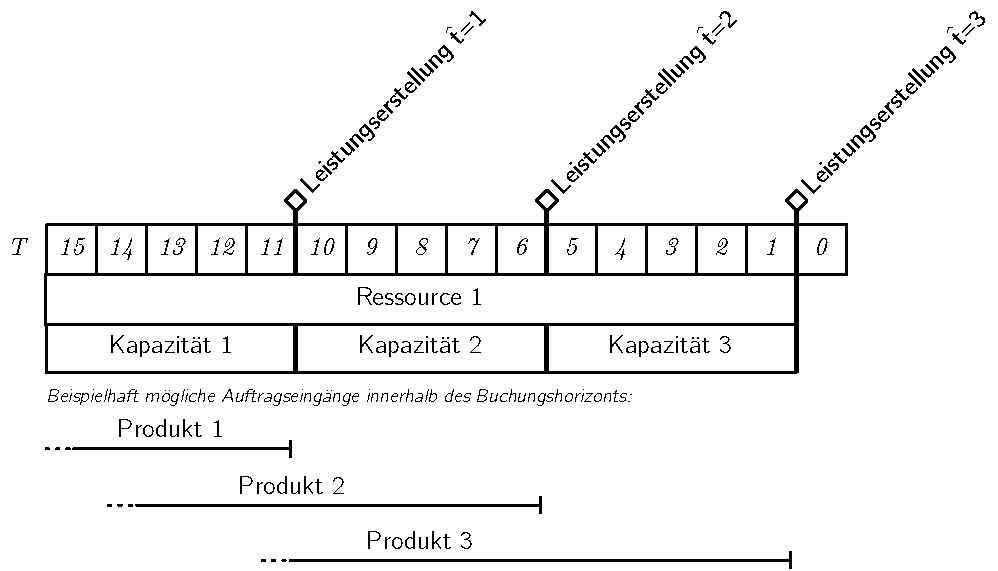
\includegraphics[width=130mm]{Bilder/Leistungsperioden2.pdf}
    \caption{Zusammenhand von Buchungsperioden und den Leistungserstellungszeitpunkten}  \label{LP2}
    {\footnotesize \textbf{In Anlehnung an:} \cite{lars}}. 
  \end{center}
\end{figure}



\section{Mathematische Formulierung eines Modells zur Entscheidungsunterstützung bei Auftragsannahme- und Lagerhaltungsentscheidungen}\label{Umformung}

% Neuer Terme
Für die Modellerweiterung erfolgt die Anpassung der \textit{Bellman'schen Funktionsgleichung}  \eqref{DP} um die Entscheidung der Lagerentnahme in Form des Terms $r_{j} + V(\textbf{c}^{\hat t}, \textbf{y}^{\hat t}-Y(\textbf{a}_j^{\hat t}, \hat t), t-1)$. Der Term beschreibt die Annahme mittels des Lagerbestands. Damit ist es dem Unternehmen möglich entweder die Kapazität oder den Lagerbestand zur Annahme einer Anfrage eines Instandhaltungsprozess in Anspruch zu nehmen. Die Entscheidung der gewollten Ablehnung einer Anfrage $j$ zur Produktion eines Lagerbestand $y_h^{\hat t}$ wird mit dem Term $V(\textbf{c}^{\hat t}-\textbf{a}^{\hat t}_j, \textbf{y}^{\hat t}+Y(\textbf{a}^{\hat t}_j, \hat t +1), t-1)$ dargestellt. Für das Modellformulierung gilt weiterhin, dass eine Ressource und eine Einheit des Lagerbestands im gleichen Verhältnis substituierbar sind.
%Eine Lagerproduktion in der Instandhaltung kann z. B. die vorherige Aufarbeitung von Ressourcen sein, damit für spätere Instandhaltungsaufträge anstelle der Instandsetzung ein Austausch des zu reparierenden Produkts erfolgt.

Sofern eine Reduzierung des Lagerbestand $\textbf{y}^{\hat t}$ als Entscheidung gewählt ist, wird der Lagerparameter bzw. die einzelnen Eintragungen des Vektors des Lagerparameters für alle betreffenden Leistungserstellungszeitpunkte $\hat t\in \hat T$ reduziert. Weiter ist dem Modell gestattet, eine Entscheidung über die Ablehnung einer Anfrage $j$ zu berücksichtigen, bei der aufgrund einer Reduktion der Ressourcenkapazität $\textbf{c}^{\hat t}$ eine Erhöhung des Lagerbestand $\textbf{y}^{\hat t}$ um jeweils des Parameters $\textbf{a}_j^{\hat t}$ möglich ist. Eine Erhöhung des Lagerbestands $\textbf{y}^{\hat t}$ einer jeden Ressource $h$ erfolgt über den gesamten Buchungshorizont und ist ab dem nachfolgenden Leistungserstellungszeitpunkt $\hat t$ verfügbar. %Sei der aktuelle Lagerbestands $\textbf{y}^{\hat t}=(0,0,0)$ über alle Leistungserstellungszeitpunkte $\hat t$. Dann erfolgt durch die Annahme einer Anfrage $j$ mit der Bestandsveränderung $\textbf{a}_j^{\hat t}=(0,1,0)$ eine Erhöhung des Lagerbestand auf $\textbf{y}^{\hat t}=(0,1,1)$, da die Leistung erst nach Erstellung in $\hat{t}=1$ verfügbar ist.

Zur Ermittlung der Veränderung des Lagerbestands aufgrund der Lagerentnahme oder der Lagerproduktion ist die Hilfsfunktion $Y(\textbf{a}_j^{\hat t}, \hat t)$ erforderlich, die den Parameter für den Kapazitätsverbrauch $\textbf{a}_j^{\hat t}$ über alle nachfolgenden Leistungserstellungszeitpunkten kumuliert.\footnote{Vgl. \cite{lars}.} Als Beispiel wird der Kapazitätsverbrauch $\textbf{a}_j^{\hat t}=(0,1,1,0)$ betrachtet. Ein Auftrag $j$ mit einem Verbrauch des vorher aufgeführten Parameters $\textbf{a}_j^{\hat t}$ zeigt eine Leistungserstellung über mehrere Perioden auf. Die Hilfsfunktion zur Ermittlung der Lagerbestandsveränderung berechnet damit eine Veränderung in Höhe des Vektors $Y(\textbf{a}_j^{\hat t}, \hat t)=(0,1,2,2)$. Sofern es sich um eine Veränderung in Form einer Lagerproduktion handelt, ist der Lagerbestand erst zur nachfolgenden Leistungserstellungsperiode $\hat t+ 1$ verfügbar. D. h. die Hilfsfunktion erstellt dem Vektor $Y(\textbf{a}_j^{\hat t}, \hat t +1 )=(0,0,1,2)$. Es muss beachtet werden, dass ein Auftrag $j$ mit einem Kapazitätsverbrauch von $\textbf{a}_j=(0,0,1,2)$ eine Lagererhöhung $Y(\textbf{a}_j, \hat t +1)=(0,0,0,1)$ verursacht. Diese Erhöhung liegt außerhalb des Betrachtungszeitraums. Damit kann zwar ein Teil der Bestandsveränderung für den aktuellen Betrachtungszeitraum genutzt werden, aber der andere Teil geht in dieser Modellformulierung verloren. Eine zusätzliche Betrachtung einer Beanspruchung von Beständen außerhalb des Betrachtungszeitraums (Perioden $t\le0$) in Form von z. B. Lagerentnahmen findet in dieser Arbeit keine Anwendung.

Die mathematische Formulierung der \textit{Bellman'schen Funktionsgleichung} für Auf\-trags\-annahme- und Lagerhaltungsentscheidungen bei auftragsbezogenen Instandhaltungsprozessen wird damit wie folgt beschrieben:
\begin{equation}\label{time}
\begin{alignat*}{2}
V(\textbf{c}^{\hat{t}}, \textbf{y}^{\hat{t}}, t) =\;& \sum_{j \in \mathcal{J}}p_{j}(t)\max[\underbrace{V(\textbf{c}^{\hat{t}}, \textbf{y}^{\hat{t}}, t-1)}_{\text{Ablehnung}}, \underbrace{r_{j} + V(\textbf{c}^{\hat{t}}-\textbf{a}^{\hat t}_j, \textbf{y}^{\hat{t}}, t-1)}_{\text{Annahme via Kapazität}},\\
& \underbrace{r_{j} + V(\textbf{c}^{\hat{t}}, \textbf{y}^{\hat{t}}-Y(\textbf{a}_j^{\hat t},\hat t), t-1)}_{\text{Annahme via Lagerentnahme}}, \underbrace{V(\textbf{c}^{\hat{t}}-\textbf{a}_j^{\hat t}, \textbf{y}^{\hat{t}}+Y(\textbf{a}_j^{\hat t}, \hat t +1), t-1)}_{\text{Ablehnung und Lagerproduktion}}]\\
& + p_{0}(t)\max_{j\in \mathcal{J},\atop p_j(t)>0}[ \underbrace{V(\textbf{c}^{\hat{t}}, \textbf{y}^{\hat{t}}, t-1)}_{\text{Keine Lagerproduktion}},  \underbrace{V(\textbf{c}^{\hat{t}}-\textbf{a}^{\hat t}_j, \textbf{y}^{\hat{t}}+Y(\textbf{a}_j^{\hat t},\hat t +1 ), t-1)}_{\text{Lagerproduktion}}]
\end{alignat*}
\end{equation}

Die Gleichung \eqref{time} zeigt im ersten Term, welche Entscheidungen bzgl. der optimalen Politik möglich sind, sofern eine Anfrage $j\in\mathcal J$ in Abhängigkeit der Wahrscheinlichkeitsverteilung $p_j(t)$ eintrifft. Es wird das Maximum über die Entscheidungen \glqq Ablehnung des Auftrags{\grqq}, \glqq Annahme via Kapazität{\grqq}, \glqq Annahme via Lagerentnahme{\grqq} sowie \glqq Lagerproduktion{\grqq} gewählt. Damit geht aus der Gleichung \eqref{time} hervor, dass es zu jedem Erwartungswert, somit für jedes Teilproblem des Netzwerks, für eine jede Anfrage $j$ die vier Optionen bzw. Entscheidungen existieren. Es gibt damit für eine jede Produktanfrage $j$ im gesamten Netzwerk einen Wert, der die optimale Politik beim Eintreffen einer Anfrage beschreibt. Dieser Wert der optimalen Politik beschreibt die Variable $d_j({\textbf{c}^{\hat t},\textbf{y}^{\hat t},t})\forall j\in\mathcal{J}$. Dieser Variable existiert für jedes Produkt und ist abhängig vom Systemzustand. Ein Systemzustand wird durch die verbleibende Kapazität $\textbf{c}^{\hat t}$ und des Lagerbestands $\textbf{y}^{\hat t}$ zur Periode $t$ beschrieben. Die Variable kann ebenfalls als Vektor $\textbf{d}({\textbf{c}^{\hat t},\textbf{y}^{\hat t},t})$ interpretiert werden und zeigt damit für ein Teilproblem des Netzwerks die optimale Politik über alle möglichen Anfragen. Inhalt des Vektors ist der jeweilige Index der optimalen Politik. Die Variable nimmt den Wert $d_j({\textbf{c}^{\hat t},\textbf{y}^{\hat t},t})=1$ an, sofern die Option der Auftragsannahme via Kapazität den höchsten Erwartungswert liefert und den Wert $d_j({\textbf{c}^{\hat t},\textbf{y}^{\hat t},t})=2$, wenn die Auftragsannahme via Lagerbestand der optimalen Politik entspricht. Sofern die Ablehnung des Auftrags erfolgen soll, aber inkl. der Entscheidung der Lagerproduktion, dann nimmt die Variable $d_j({\textbf{c}^{\hat t},\textbf{y}^{\hat t},t})$ den Wert $3$ an. Sofern die optimale Politik die generelle Ablehnung der Anfrage ist, nimmt die Variable den Wert $d_j({\textbf{c}^{\hat t},\textbf{y}^{\hat t},t})=0$ an.

% Alte und neue Grenzbedingungen
Für die verschiedenen Entscheidungsalternativen existieren unterschiedliche $OC_{j}$, wie aus der Gleichung \eqref{time} zu erkennen ist. Damit trägt der Parameter $OC_{j}$ den Superskript $d$ für die jeweilig möglichen Entscheidungsalternative aufgrund der Modellformulierung. In dieser Modellerweiterung existieren vier unterschiedliche Entscheidungen, die den möglichen Ausprägungen der optimalen Politik der Variable $d_{j}(\textbf{c}^{\hat t},\textbf{y}^{\hat t},t)$ entsprechen. Sofern die verschiedenen möglichen Entscheidungen im betrachteten Systemzustand gleichwertig sind, was abhängig von den Parametern $r_{j}$ und $OC_j^{d}$ ist, wird die Annahme einer Anfrage über die Ressourcenkapazität bevorzugt. Anschließend erfolgt die Bevorzugung der Annahme einer Anfrage via Lagerbestand, falls die anderweitigen Entscheidungen einen gleichwertigen Wert aufweisen.

Es gelten die Grenzbedingungen \eqref{GB1} sowie \eqref{GB2} aus Kapitel \ref{KapitelDP} und bzgl. der optimalen Politik zur Annahme von Anfragen nach Produkt $j$ gilt folgende Annahme:
\begin{equation}\label{GB3}
     d_{j}({\textbf{c}^{\hat t},\textbf{y}^{\hat t}, t}):=\left\{\begin{array}{llll}
     1, & \text{für } r_{j} - OC_{j}^{1} \ge r_{j} - OC_{j}^{2}\\
         2, & \text{für } r_{j} - OC_{j}^{2} \ge -OC_{j}^{3}\\
         3, & -OC_{j}^{3} > 0\\
         0, & \text{sonst}\end{array}\right. .
\end{equation}

Die \textit{Bellman'schen Funktionsgleichung} \eqref{time} zeigt ebenfalls den Term an, sofern keine Anfrage eintrifft. Bei der Auftragsannahme von Kundenaufträgen unter Berücksichtigung von Lagerhaltungsentscheidung muss beachtet werden, dass auch Entscheidungsalternativen beim Einreffen keiner Produktanfragen $j\in\mathcal{J} $ bestehen. Sofern keine Anfrage eintrifft, gibt es die Entscheidung über alle möglichen Produktanfragen $j\in\mathcal{J}$ die Lagerproduktion durch Inanspruchnahme der Kapazitäten durchzuführen. Damit existiert auch eine optimale Politik, sofern keine Anfrage $j\in\mathcal{J}$ zur Periode $t$ eintrifft. Für diese optimale Politik wird die Variable $d_0({\textbf{c}^{\hat t},\textbf{y}^{\hat t},t})$ verwendet. Es bestehen die gleichen Abhängigkeiten wie bei der Variable für die optimale Politik bei Auftragseingang ($d_j({\textbf{c}^{\hat t},\textbf{y}^{\hat t},t})$). Die Variable zeigt jedoch nicht einen Index über die optimale Entscheidung, sonder sie zeigt den Index der Produktanfrage $j$ die für die Lagerproduktion durch Verwendung des zugehörigen Ressourceneinsatzes bzw. Ausführungsmodus $\textbf a_j$ verwendet werden soll. Sofern keine Lagerproduktion die optimale Politik ist, nimmt die Variable den Wert $0$ an. Dabei wird für der optimalen Politik $d_0({\textbf{c}^{\hat t},\textbf{y}^{\hat t},t})$ zur Vereinfachung des Modells angenommen, dass nur dann eine Lagererhöhung erfolgen kann, sofern Anfragen nach Produkten $j\in\mathcal J$ möglich sind ($p_j(t)>0$). Damit wird die Variable wie folgt definiert:
\begin{equation}\label{GB4}
     d_{0}({\textbf{c}^{\hat t},\textbf{y}^{\hat t}, t}):=\left\{\begin{array}{ll}
         j, & \text{für }\{ j\; |\; \max_{\substack{j\in \mathcal{J},\\ p_j(t)>0}} -OC_{j}^{3}\}\\
         0, & \text{sonst}\end{array}\right. .
\end{equation}



Im nachfolgenden Schritt kann die Gleichung \eqref{time} analog der Gleichung \eqref{DP} umgeformt werden:
%Umformung
\begin{equation}\label{time2}
\begin{alignat*}{2}
V(\textbf{c}^{\hat{t}}, \textbf{y}^{\hat{t}}, t) = \;& \sum_{j \in \mathcal{J}}p_{j}(t)V(\textbf{c}^{\hat{t}}, \textbf{y}^{\hat{t}}, t-1) + \sum_{j \in \mathcal{J}}p_{j}(t)\max[0, \\
& r_{j} - V(\textbf{c}^{\hat{t}}, \textbf{y}^{\hat{t}}, t-1)+ V(\textbf{c}^{\hat{t}}-\textbf{a}^{\hat t}_j, \textbf{y}^{\hat{t}}, t-1), \\
& r_{j} - V(\textbf{c}^{\hat{t}}, \textbf{y}^{\hat{t}}, t-1) + V(\textbf{c}^{\hat{t}}, \textbf{y}^{\hat{t}}-Y(\textbf{a}^{\hat t}_j,\hat t), t-1),\\
& V(\textbf{c}^{\hat{t}}-\textbf{a}_j^{\hat t}, \textbf{y}^{\hat{t}}+Y(\textbf{a}_{j}^{\hat t}, \hat t+1), t-1) - V(\textbf{c}^{\hat{t}}, \textbf{y}^{\hat{t}}, t-1) ]\\
&+p_{0}(t)V(\textbf{c}^{\hat{t}}, \textbf{y}^{\hat{t}}, t-1)\\
& + p_{0}(t)\max_{j\in \mathcal{J},\atop p_j(t)>0}[0, V(\textbf{c}^{\hat{t}}-\textbf{a}_j^{\hat t}, \textbf{y}^{\hat{t}}+Y(\textbf{a}_j^{\hat t},\hat t +1 ), t-1)\\
&- V(\textbf{c}^{\hat{t}}, \textbf{y}^{\hat{t}}, t-1)]\\[10pt]
= \;& V(\textbf{c}^{\hat{t}}, \textbf{y}^{\hat{t}}, t-1) + \sum_{j \in \mathcal{J}}p_{j}(t)\max[0, \\
& r_{j} - V(\textbf{c}^{\hat{t}}, \textbf{y}^{\hat{t}}, t-1)+ V(\textbf{c}^{\hat{t}}-\textbf{a}_j^{\hat t}, \textbf{y}^{\hat{t}}, t-1), \\
& r_{j} - V(\textbf{c}^{\hat{t}}, \textbf{y}^{\hat{t}}, t-1) + V(\textbf{c}^{\hat{t}}, \textbf{y}^{\hat{t}}-Y(\textbf{a}_j^{\hat t},\hat t), t-1),\\
& V(\textbf{c}^{\hat{t}}-\textbf{a}_j^{\hat t}, \textbf{y}^{\hat{t}}+Y(\textbf{a}_{j}^{\hat t}, \hat t +1), t-1) - V(\textbf{c}^{\hat{t}}, \textbf{y}^{\hat{t}}, t-1) ]\\
& + p_{0}(t)\max_{j\in \mathcal{J},\atop p_j(t)>0}[0, V(\textbf{c}^{\hat{t}}-\textbf{a}^{\hat t}_j, \textbf{y}^{\hat{t}}+Y(\textbf{a}^{\hat t}_j, \hat t +1), t-1)\\
& - V(\textbf{c}^{\hat{t}}, \textbf{y}^{\hat{t}}, t-1)]
\end{alignat*}
\end{equation}

%Aufbauen auf den vorhergehenden Erweiterung erfolgt die Betrachtung des Modells um eine andere Möglichkeit der Lagerhaltungsentscheidung.
Die Beschreibung der Funktionsweise der Modellerweiterung wird anhand nachfolgendem Beispiels getätigt:

\begin{center}
$j = \{1, 2, 3\}, \; h = \{1\}, \; r_{1} = 100, \; r_{2} = 200, \; r_{3} = 5000,$ \\
$\text{Startperiode } t=3, \; \text{Anzahl Leistungserstellungen } \hat{T}= 3$,
\end{center}
\[
    \textbf{c}^{\hat{t}}=\begin{pmatrix} 1\\ 1\\ 1  \end{pmatrix}, \;
    \textbf{a}^{\hat t}_{1}=\begin{pmatrix} 1\\ 0\\ 0  \end{pmatrix}, \;
     \textbf{a}^{\hat t}_{2}=\begin{pmatrix} 0\\ 1\\ 0  \end{pmatrix}, \;
       \textbf{a}^{\hat t}_{3}=\begin{pmatrix} 0\\ 0\\ 2  \end{pmatrix}, \;
            p_{j}(t)=
       \begin{pmatrix}
       0.3 & 0 & 0 \\
0.3 & 0.3 & 0 \\
0.3 & 0.3 & 0.3
\end{pmatrix}, 
  \]
  \[
    \textbf{y}^{\hat t}= \begin{pmatrix} 0\\ 0\\ 0  \end{pmatrix}, \;
    \textbf{y}^{\hat t, max}=\begin{pmatrix} 2\\ 2\\ 2  \end{pmatrix}
      \]
      
Bei dem Beispiel wird ein Netzwerk mit drei Produktanfragen $j\in\mathcal{J}$ betrachtet. Es existieren drei Leistungserstellungszeitpunkte $\hat t$ für eine Ressource $h\in\mathcal{H}$. Die Annahmen der Produktanfragen $j\in\mathcal{J}$ generieren einen Ertrag in Höhe von $r_1=100, r_2=200$ und $r_3=5000$. Die Kapazitäten für die Ressourcen betragen $\textbf{c}^{\hat t}=(1,1,1)$ und die Bestandsveränderungen für die Anfragen betragen $\textbf{a}^{\hat t}_1=(1,0,0),\; \textbf{a}^{\hat t}_2=(0,1,0)$ sowie $\textbf{a}^{\hat t}_3=(0,0,2)$. Der Buchungshorizont beträgt $T=3$. Es existiert kein Lagerbestand $\textbf{y}^{\hat t}$ und es kann nur ein maximaler Lagerbestand $\textbf{y}^{\hat t, max}=(2, 2, 2)$ zu jeder Leistungserstellung aufgebaut werden. In diesem Beispiel sind nicht alle Produktanfragen $j\in\mathcal{J}$ zu jedem Zeitpunkt $t\in T$ möglich. Dies zeigt die Matrix $p_{j}(t)$ mit den Eintrittswahrscheinlichkeiten für jedes Produkt $j$ zum jeweiligen Zeitpunkt $t$. Für das Produkt $j=1$ treffen Anfragen zu den Zeitpunkten $t\in T$ mit den Wahrscheinlichkeiten $p_{1}(t)=(0.3, 0, 0)$ ein. Für die Produkte $j=2$ und $j=3$ betragen die Wahrscheinlichkeiten $p_{2}(t)=(0.3, 0.3, 0)$ bzw. $p_{3}(t)=(0.3, 0.3, 0.3)$. Bei den Wahrscheinlichkeiten $p_j(t)$ der Produktanfrage $j$ zum Zeitpunkt $t$ muss beachtet werden, dass der Buchungshorizont rückwärts verläuft. Abbildung \ref{B9} zeigt für das Beispiel die möglichen Systemzustände mit allen Übergängen. Dabei wird ein Systemzustand im Netzwerk als Zahlenfolge $[c^{\hat t=1}_1\;c^{\hat t=2}_1\;c_1^{\hat t=3}\;y_1^{\hat t=1}\;y_1^{\hat t=2}\;y_1^{\hat t=3}\;t]$ beschrieben.

\begin{figure}[h!]
  \begin{center}
    \includegraphics[width=200mm, angle=90]{Bilder/Beispiel9.pdf}
    \caption{Darstellung der Systemzustände des Netzwerk RM unter Beachtung der Möglichkeit der Auftragsannahme- und Lagerhaltungsentscheidung}  \label{B9}
    {\footnotesize \textbf{Legende:} Die Zahlen stehen für den Auftrag $j$, AA='Auftragsannahme', LE='Lagerentnahme', LP='Lagerproduktion', KA='Kein Auftrag', $\cdots$='Anfrage ablehnen'.} 
  \end{center}
\end{figure}

Wie in der Abbildung \ref{B9} zu erkennen ist, wäre die optimale Politik $d_{j}({\textbf{c},\textbf{y}, t})$ im Systemzustand $[1\;1\;1\;0\;0\;0\;3]$ eine Produktanfrage $j=1$ abzulehnen und eine Bestandsveränderung des Lagers zu bewilligen (Lagerproduktion) sowie die Annahme der Produktanfrage $j$ anhand der vorhandenen Kapazität. Eine Anfrage $j=3$ kann in diesem Systemzustand nicht akzeptiert werden, da nicht genügend Kapazität vorhanden ist und daher wird der Übergang in einem Systemzustand mit einer negativen Ressourcenkapazität nicht dargestellt. Sofern eine Anfrage $j=1$ im Systemzustand $[1\;1\;1\;0\;0\;0\;3]$ eintrifft, ist die optimale Politik die Lagerproduktion unter Verwendung der Kapazitäten. Damit erreicht das Netzwerk den Systemzustand $[0\;1\;1\;0\;1\;1\;2]$. Erkennbar ist, dass die Reduktion der Kapazität $c_1^{\hat t=1}$ auf $0$ erfolgt und nach dem Leistungserstellungszeitpunkt $\hat t = 1$ ein Lagerbestand $\textbf y^{\hat t}$ zur Verfügung steht. Eine Auftragsannahme der Anfrage $j=1$ gehört in diesem Netzwerk nicht zur optimalen Politik.

Im Systemzustand $[0\;1\;1\;0\;1\;1\;2]$ ist aufgrund der Wahrscheinlichkeitsverteilung $p_j(t)$ keine Anfrage nach Produkt $j=1$ mehr möglich und ebenfalls ist eine Annahme einer Anfrage nach Produkt $j=3$ aufgrund der Kapazitätsbestände ausgeschlossen. In diesem Systemzustand ist, sofern die Anfrage eintrifft, das Ablehnen inkl. einer Lagerproduktion der Produktanfrage $j=2$ alleiniger Bestandteil der optimalen Politik. Aufgrund einer solchen Entscheidung erfolgt der Übergang in den Systemzustand $[0\;0\;1\;0\;1\;2\;1]$. Wie die Zahlenfolge $[0\;0\;1\;0\;1\;2\;1]$ des Systemzustands andeutet, ist anhand des Lagerhaltungsparameters $\textbf y^{\hat t}=(0,1,2)$ erstmalig eine Annahme der Produktanfrage $j=3$ möglich. Sofern diese aufgrund der Wahrscheinlichkeitsverteilung $p_j(t)$ einzig mögliche Anfrage eintrifft, ist die optimale Politik des Netzwerks die Annahme der Anfrage $j=3$ anhand der Entscheidung der Lagerentnahme ($d_{3}((0,0,1)^{\textnormal T},(0,1,2)^{\textnormal T}, 1)=2$). Erfolgt eine solche Reihenfolge des Eintreffens der Auftrage, dann würde ein Unternehmen unter Einhaltung der optimalen Politik ein Gesamtertrag in Höhe von $5000$ GE erzielen.

Sofern im Ausgangssystemzustand $[1\;1\;1\;0\;0\;0\;3]$ eine Anfrage nach einem Produkt $j=2$ eintrifft, ist die optimale Politik die Annahme der Anfrage über die Ressourcenkapazitität $\textbf{c}^{\hat t}$. Aufgrund dieser Entscheidung ist ein Gesamtertrag in Höhe von $200$ GE erzielt. Eine Entscheidung über die Lagerproduktion unter diesen Parametergegebenheiten hätte in Bezug der Zielsetzung der Maximierung des Gesamtdeckungsbeitrags keinen weiteren Nutzen. Wie in der Abbildung \ref{B9} zu erkennen ist, würde eine Lagerproduktion zwar den Bestand an Ressourcen auf Lager erhöhen, jedoch wäre im weiteren Verlauf keine Annahme einer anderen Produktanfrage $j\in\mathcal J$ möglich. %Sofern ein Unternehmen sich gegen die optimale Politik entscheidet, würde kein Ertrag im weiteren Verlauf des Netzwerks generiert.

\begin{table}
\begin{footnotesize}
     \caption{Optimale Politik für das beispielhafte Netzwerk RM unter Beachtung von Auftragsannahme- und Lagerhaltungsentscheidungen} \label{Tab9}
    \vspace*{3mm}
        \begin{center}
\csvautotabular{data/beispiel9.csv}
      \end{center}
    \begin{center}
      %{\footnotesize \textbf{Legende:} LE='Lagerentnahme', LP='Lagerproduktion', KA='Kein Auftrag'} 
      \end{center}
\end{footnotesize}
\end{table}

Trifft im Ausgangssystemzustand $[1\;1\;1\;0\;0\;0\;3]$ keine Anfrage $j$ ein, dann ist die optimale Politik $d_{0}({\textbf{c}^{\hat t},\textbf{y}^{\hat t}, t})=1$. D. h. sofern keine Anfrage $j\in\mathcal{J}$ zur Periode $t=3$ eintrifft, wäre es die optimale Politik des Unternehmens den Parameter der Bestandsveränderung $\textbf{a}_j$ der Produktanfrage $j=1$ zu verwenden, damit sich der Lagerbestand $\textbf{y}^{\hat t}$ ab der Leistungsperiode $\hat{t}=2$ um eine Einheit erhöht. Anders formuliert, das Unternehme sollte die vorhandene Kapazität nicht verfallen lassen und eine Lagerproduktion veranlassen. Die weitere optimale Politik für dieses Netzwerk ist, sofern keine Produktanfragen eintreffen, das Verfolgen einer optimalen Politik, die eine Annahme der Produktanfrage $j=3$ zur letzten Periode $t$ ermöglicht. Tabelle \ref{Tab9} zeigt zusammenfassend die berechneten Erwartungswerte und die optimale Politik für alle Systemzustände des Beispiels.

Die eigentliche Funktionsweise des hier vorgestellten Modells geht anhand des vorher aufgeführten Beispiels jedoch teilweise verloren, da die Anzahl an Buchungsperioden $t\in T$ der Anzahl der möglichen Buchungsabschnitte $\hat{t}\in\hat{T}$ entspricht. Zur besseren Veranschaulichung wird ein umfangreicheres Beispiel berechnet:

{\begin{center}
$j = \{1, 2, 3, 4\}, \; h = \{1\}, \; r_{1} = 100, \; r_{2} = 5000, \; r_{3} = 100, \; r_{4} = 5000,$ \\
$\text{Startperiode } t=10, \; \text{Anzahl Leistungserstellungen } \hat{T}= 3  $,
\[\textbf{c}^{\hat{t}}=\begin{pmatrix} 1\\ 1  \end{pmatrix}, \;
    \textbf{a}^{\hat t}_1=\begin{pmatrix} 1\\ 0  \end{pmatrix}, \;
\textbf{a}^{\hat t}_2=\begin{pmatrix} 1\\ 0  \end{pmatrix}, \;
\textbf{a}^{\hat t}_3=\begin{pmatrix} 0\\ 1  \end{pmatrix}, \;
\textbf{a}^{\hat t}_4=\begin{pmatrix} 0\\ 1  \end{pmatrix}, \]
         \[ p_{j}(t)=
       \begin{pmatrix}
       0.2 & 0.2 & 0.2 & 0.2 & 0.2 & 0 & 0 & 0 & 0 & 0\\
       0.2 & 0.2 & 0.2 & 0.2 & 0.2 & 0 & 0 & 0 & 0 & 0\\
       0.2 & 0.2 & 0.2 & 0.2 & 0.2 & 0.2 & 0.2 & 0.2 & 0.2 & 0.2\\
       0.2 & 0.2 & 0.2 & 0.2 & 0.2 & 0.2 & 0.2 & 0.2 & 0.2 & 0.2
\end{pmatrix}, 
  \]
  \[
    \textbf{y}^{\hat t}= \begin{pmatrix} 0\\ 0\end{pmatrix}, \;
    \textbf{y}^{\hat t, max}=\begin{pmatrix} 1\\ 1  \end{pmatrix}
      \]
\end{center}}

Für dieses Beispiel ist eine grafische Auswertung unter Beachtung der Parameter und der Menge an möglichen Systemübergängen nicht mehr zielführend. Eine Auswertung der optimalen Politik anhand einer tabellarischen Auswertung ist jedoch weiterhin möglich, wie Tabelle \ref{Tab10} zeigt. Die Tabelle führt die jeweiligen Erwartungswerte und die optimalen Politik für jeden Systemzustand auf. Dabei wird in diesem Beispiel ein Systemzustand als Zahlenfolge $[c_1^{\hat t=1}\;c_1^{\hat t=2}\;y_1^{\hat t=1}\;y_1^{\hat t=2}\;t]$ definiert.

\begin{table}
\renewcommand{\arraystretch}{1}
\begin{footnotesize}
     \caption{Optimale Politik für das zweite beispielhafte Netzwerk RM unter Beachtung von Auftragsannahme- und Lagerhaltungsentscheidungen} \label{Tab10}
        \begin{center}
\csvautotabular{data/beispiel10.csv}
      \end{center}
\end{footnotesize}
\end{table}

Wie aus der Tabelle \ref{Tab10} zu erkennen ist, ermittelt der Algorithmus keine optimale Politik der Instandsetzung von Lagerbeständen für die Aufträge $j=3$ und $j=4$. Dies liegt daran, dass die Bereitstellung des aufgewerteten Lagerbestands erst außerhalb des Buchungshorizonts $T$ verfügbar ist. Es liegt eine Dominanz der Annahmen von $j=2$ bzw. $j=4$ für das gesamte Netzwerk vor, sofern die Wahrscheinlichkeit des Auftragseingangs besteht. Zur den anfänglichen Buchungsperiode gehört die Annahme der ertragsarmen Anfragen $j=1$ und $j=3$ nicht zur optimalen Politik. Jedoch könnte die Kapazität $c_{h}^{\hat t}$ der Produktanfrage $j=1$ genutzt werden, damit ein Lagerbestand $y_{h}^{\hat t}$ generiert wird. Der Lagerbestand wäre demnach nach dem Leistungserstellungszeitpunkt $\hat{t}=1$ verfügbar. Erfolgt zum Zeitpunkt $t=10$ der Auftragseingang von $j=1$, dann ist eine Annahme über die Kapazitäten jedoch nicht die optimale Politik, sonder die komplette Ablehnung des Auftrags. D. h. der Kapazitätsverbrauch $\textbf{a}^{\hat t}_j$ der Anfrage $j$ wird nicht aufgewendet um den Lagerbestand $\textbf y^{\hat t}$ um $Y(\textbf{a}^{\hat t}_j,\hat t+1)$ zu erhöhen. Die Entscheidung über eine Lagerproduktion, die aufgrund des Eingangs einer Produktanfrage $j=1$ getätigt werden kann, erfolgt erst ab der Periode $t=7$. Für das Netzwerk wandeln sich ab diesem Zeitpunkt die OK in der Form, dass eine Übertragung der Kapazität bzgl. der Zielvorgabe der Maximierung des zu erwartenden Gesamtertrags sinnvoller ist. Damit wäre ein Lagerbestand für weitere Produktanfragen $j=2$ (und $j=4$) möglich und die Kapazität $c_{h}^{\hat t}$ aus $\hat{t}=1$ wäre aufgrund des ablaufenden Buchungshorizonts weiterhin verfügbar.\\[.5cm]

Sofern keine Anfragen in dem Beispiel eintreffen, ergibt sich ein differenziertes Bild bzgl. der optimalen Politik. Sofern Kapazitäten die $c_{h}^{\hat t}$ zu den Zeitpunkten $t<5$ vollständig verfügbar sind, wird keine Lagerproduktion durchgeführt. Das Modell versucht weiter den Ertrag durch die möglichen Erträge $r_j$ der Produktnachfragen $j=2$ und $j=4$ zu maximieren. Sofern jedoch in diesem Zeitabschnitt eine Produktanfrage $j=2$ oder $j=4$ eingetroffen und dementsprechend die Kapazität reduziert ist, wird das Modell die Kapazität $c_{h}^{\hat t=1}=1$ zum Lagerbestand $y_{h}^{\hat t=2}$ umschichten. Dies erfolgt mit dem Bestandveränderungsparameter $\textbf{a}_j^{\hat t}$ für $j=1$ und nur dann, wenn keine Anfrage $j\in\mathcal{J}$ in den Zeitpunkten $t>5$ eintreffen. Damit folgt die optimale Politik $d_{0}({\textbf{c}^{\hat t},\textbf{y}^{\hat t}, t})$ der optimalen Politik $d_{j}({\textbf{c}^{\hat t},\textbf{y}^{\hat t}, t})$.


\section{Grundlegendes zum Lösen und Implementieren des Auftragsannahmeproblems}\label{Implementierung}

Gleichung \eqref{time} zeigt die mathematische Modellformulierung für das Auftragsannahmeproblem im Netzwerk RM mit Lagerhaltungsentscheidungen. In diesem Abschnitt wird ein mögliches Lösungsverfahren für das Optimierungsmodell gezeigt, damit eine Implementierung in ein Computersystem möglich ist. Mittels einer solchen Implementierung kann das exakte Lösen von vordefinierten Szenarien erfolgen. Bei der \textit{Bellman'sche Funktionsgleichung} \eqref{time} aus Abschnitt \ref{Umformung} handelt es um ein stochastisch, dynamisches Optimierungsproblem in rekursiver Form.\footnote{Vgl. \cite{Petrick:2009aa}, S. 185.} Das Optimierungsmodell besteht aus verschiedenen gleichartigen Teilproblemen und zur Lösung des gesamten Optimierungsmodells müssen alle Teilprobleme gelöst werden.\footnote{Vgl. \cite{powell2007approximate}, S. 26, 31-33.} Diese Art der rekursiven Modellformulierung geht auf das von dem amerikanischen Mathematiker Richard Bellman entwickelte Konzept der \textbf{Dynamischen Programmierung (DP)} zurück.\footnote{Vgl. \cite{bellman1954theory}, S. 4; \cite{Bellman:1952aa}, S. 716-717.} Bei diesem Konzept werden die berechneten Teilergebnisse gespeichert und bei der weiteren Berechnung des Optimierungsmodells verwendet.\footnote{Vgl. \cite{owsnicki1999algorithmen}, S. 197.} Durch eine solche Implementierung wird die rekursive Berechnung des Modells verbessert, da der Zugriff auf bereits berechnete Teilergebnisse erfolgt, sofern die einzelnen Teilergebnisse sich überlappen.

Eine Form der Implementierung des Konzepts der DP ist das Anwenden einer \textit{Memofunktion}. Mit der Memofunktion werden die bereits berechneten Lösungen des Optimierungsmodells gespeichert. Sofern die rekursive Folge auf ein bereits berechnetes Teilproblem stößt, wird auf die abgespeicherte Lösung zurückgegriffen.\footnote{Vgl. \cite{hetland2010python}, S. 176-181.} Das stochastisch, dynamisches Optimierungsmodell lässt sich als Graph interpretieren, bei dem die Knoten die Teilprobleme und die Kanten die einzelnen Übergängen in die nachfolgenden Teilprobleme sind. Zur Verdeutlichung einer Memofunktion im Netzwerk RM in der Auftragsannahme wird ein einfaches Beispiel eingeführt: $j = \{1, 2\}, \; h = \{1\}, c_{1}=2, a_{11}=1, a_{12}=1, \text{ Startperiode } t=2.$

\begin{figure}[h!]
  \begin{center}
    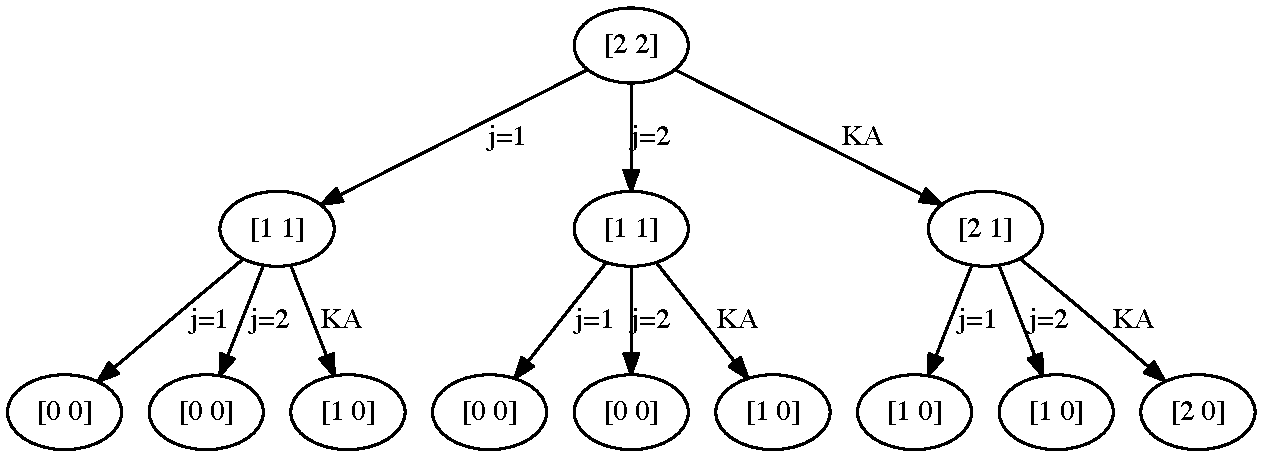
\includegraphics[width=140mm]{Bilder/Einfach.pdf}
    \caption{Rekursive Übergänge der Systemzustände ohne Memofunktion}  \label{Einfach}
        {\footnotesize \textbf{In Anlehnung an:} \cite{hetland2010python}, S. 179.} 
    {\footnotesize \textbf{Legende:} Annahme eines Produktauftrags entspricht '$j$', KA='Kein Auftrag'} 
  \end{center}
\end{figure}

Abbildung \ref{Einfach} zeigt die möglichen Systemzustände in Form der Knoten und die Übergänge in Form der Kanten. Dabei ist ein Knoten definiert als Zahlenfolge $[c_h\; t]$ und zeigt damit den Kapazitätsbestand $c_h$ zum Zeitpunkt $t$. Durch Annahme einer Produktanfrage $j\in\mathcal{J}$ oder sofern keine Anfrage eintrifft, wird ein Systemzustand verlassen. Diese rekursive Folge des Graphen wird konstruiert durch Anwenden der Gleichung \eqref{DP}. Sofern keine Memofunktion Anwendung findet, werden die einzelnen Teilprobleme jeweils mehrfach ermittelt, da sie jeweils für das vorherige Teilproblem notwendig sind.

\begin{figure}[h!]
  \begin{center}
    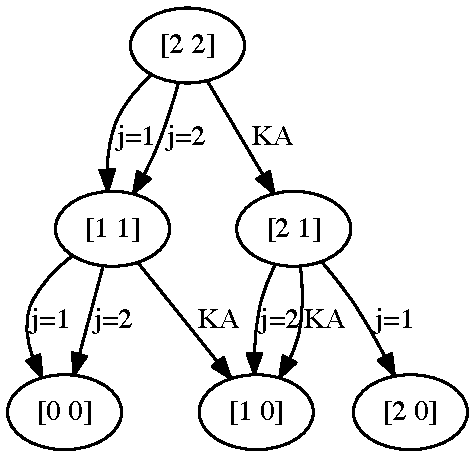
\includegraphics[width=50mm]{Bilder/Einfach2.pdf}
    \caption{Rekursive Übergänge mit Memofunktion}  \label{Einfach2}
        {\footnotesize \textbf{In Anlehnung an:} \cite{hetland2010python}, S. 179.} 
    {\footnotesize \textbf{Legende:} Annahme einer Produktauftrag entspricht '$j$', KA='Kein Auftrag'} 
  \end{center}
\end{figure}

Durch Anwenden einer Memofunktion können die möglichen Übergänge der Systemzustände des Beispiels reduziert werden, wie Abbildung \ref{Einfach2} zeigt. Jedes Systemzustand ist nur einmal im Zustandsraum vorhanden und sofern der rekursive Verlauf auf ein bereits ermitteltes Teilproblem trifft, erfolgt das Abrufen der bereits gespeicherten Lösung. Anders formuliert bedeutet dies, dass nachdem der Systemzustand bzw. das Teilproblem $[1\; 1]$ aufgrund der Anfrage nach Produkt $j=1$ gelöst ist, erfolgt keine Berechnung des gleichen Systemzustands $[1\; 1]$ aufgrund der Anfrage nach Produkt $j=2$. Das Ergebnis des Teilproblems wird direkt aus der Memofunktion abgerufen.

Der in dieser Arbeit verwendete \textbf{Algorithmus} zum exakten Lösen des Auftragsannahmeproblems im Netzwerk RM verwendet eine solche Memofunktion. Der Algorithmus berechnet den Erwartungswert des maximal möglichen Ertrags für ein Netzwerk RM auf Basis der rekursiven Form der Gleichung \eqref{time2}. Er durchläuft alle möglichen Teilprobleme bzw. Systemzustände des Netzwerks, indem der Algorithmus sich selbst mit angepassten Parametern aufruft. Als Grenzen für die rekursive Abfolge werden die Grenzbedingungen \eqref{GB1} und \eqref{GB2} hinterlegt. Das Lösen des Optimierungsproblems erfolgt damit durch Rückwärtsinduktion der rekursiven Folge, wobei bei jedem Teilproblem geprüft wird, ob bereits eine Lösung in der Memofunktion vorliegt. Nachfolgend wird der verwendete Algorithmus als Pseudocode dargestellt.


\begin{algorithm}[H]
%\renewcommand{\lstlistingname}{Code}
\textbf{Pseudocode: Auftragsannahmeproblem im Netzwerk RM;\\ 
Ermittlung des Erwartungswerts $V(\textbf{c}^{\hat t},\textbf{y}^{\hat t},t)$}\\
\Ein{$Memofunktion$}
\Ein{$\mathcal{H}$, $\mathcal{J}$, $T$, $\hat T$, $\textbf{c}^{\hat t}$, $\textbf{y}^{\hat t}$, $\textbf{a}^{\hat t}_j$, $r_{j}$, $p_j(t)$}
\uWenn{$V(\textnormal{\textbf c}^{\hat t},\textnormal{\textbf y}^{\hat t},t) \notin Memofunktion$}{
	\uWenn{$t \neq 0$}{
		$value^{reject} = V(\textbf{c}^{\hat t},\textbf{y}^{\hat t},t-1)$\\
		\FuerJedes{$j\in\mathcal{J}$}{
		% Accept
			\uWenn{$\textnormal{\textbf c}^{\hat t}-\textnormal{\textbf a}_j^{\hat t}\ge \textnormal{\textbf{0}}$}{
				$value_{j}^{accept} = p_j(t)\cdot\max[0,r_{j}-value^{reject}+V(\textnormal{\textbf c}^{\hat t}-\textnormal{\textbf a}^{\hat t}_j,\textbf{y}^{\hat t},t-1)]$}
			\uSonst{Grenzbedingung \eqref{GB2}: $V(\textnormal{\textbf c}^{\hat t}-\textnormal{\textbf a}^{\hat t}_j,\textbf{y}^{\hat t},t-1)=-\infty$\\
			$value_{j}^{accept} = p_j(t)\cdot\max[0,r_{j}-value^{reject}-\infty]$}
			% 2
			\uWenn{$\textnormal{\textbf y}^{\hat t}-Y(\textnormal{\textbf a}_j^{\hat t},\hat t)\ge \textnormal{\textbf{0}}$}{
				$value_{j}^{storage} = p_j(t)\cdot\max[0,r_{j}-value^{reject}+V(\textnormal{\textbf c}^{\hat t},\textbf{y}^{\hat t}-Y(\textnormal{\textbf a}^{\hat t}_j,\hat t),t-1)]$}
			\uSonst{Grenzbedingung \eqref{GB2}: $V(\textnormal{\textbf c}^{\hat t},\textbf{y}^{\hat t}-Y(\textnormal{\textbf a}^{\hat t}_j,\hat t),t-1)=-\infty$\\
			$value_{j}^{storage} = p_j(t)\cdot\max[0,r_{j}-value^{reject}-\infty]$}
				% 3
			\uWenn{$\textnormal{\textbf c}^{\hat t}-\textnormal{\textbf a}_j^{\hat t}\ge \textnormal{\textbf{0}} \textnormal{\textbf{ and }} \textnormal{\textbf y}^{\hat t}+Y(\textnormal{\textbf a}_j^{\hat t},\hat t +1)\le \textnormal{\textbf{y}}^{\hat t, max}$}{
				$value_{j}^{workup} = p_j(t)\cdot\max[0,V(\textnormal{\textbf c}^{\hat t}-\textnormal{\textbf a}^{\hat t}_j,\textbf{y}^{\hat t}+Y(\textnormal{\textbf a}_j^{\hat t},\hat t+1),t-1)-value^{reject}]$}
			\uSonst{Grenzbedingung \eqref{GB2}: $V(\textnormal{\textbf c}^{\hat t}-\textnormal{\textbf a}^{\hat t}_j,\textbf{y}^{\hat t}+Y(\textnormal{\textbf a}_j^{\hat t},\hat t+1),t-1)=-\infty$\\
			$value_{j}^{workup} = p_j(t)\cdot\max[0,-\infty-value^{reject}]$}
			
			}
			$list = [0]$\\
			\FuerJedes{$j\in\mathcal{J}$}{
			\uWenn{$p_j(t)>0$}{
			$list = list + [V(\textnormal{\textbf c}^{\hat t}-\textnormal{\textbf a}^{\hat t}_j,\textbf{y}^{\hat t}+Y(\textnormal{\textbf a}_j^{\hat t},\hat t+1),t-1)-value^{reject}]$
			}\uSonst{$list = list + [0]$}}
			
		$V(\textbf{c}^{\hat t},\textbf{y}^{\hat t},t)=value^{reject} + \sum_{j\in\mathcal{J}}(value_j^{accept}+value_j^{storage}+value_j^{workup})+p_0(t)\max [list]$}
	\uSonst{Grenzbedingung \eqref{GB1}: $V(\textbf{c}^{\hat t},\textbf{y}^{\hat t},t)=0$}
	$Memofunktion = Memofunktion+[V(\textbf{c}^{\hat t},\textbf{y}^{\hat t},t)]$}
\lSonst{$V(\textbf{c}^{\hat t},\textbf{y}^{\hat t},t) \textbf{ aus } Memofunktion$}
\Aus{$V(\textbf{c}^{\hat t},\textbf{y}^{\hat t},t)$}
%{\footnotesize \textbf{Quelle:} \cite{bouleimen2003new}, S. 273}
\end{algorithm}

Bei der Implementierung des Algorithmus zum Lösen der Modellerweiterung des Auftragsannahmeproblems im Netzwerk RM mit Lagerhaltungsentscheidungen wurde die Programmiersprache \texttt{Python/2.7.1} verwendet. Es handelt sich um eine höhere Programmiersprache mit einem Interpreter.\footnote{Vgl. \cite{:2005aa}, S. 8.} Als  Kommandozeileninterpreter wird in dieser Arbeit \texttt{IPython/3.2.1} genutzt. Zur Verbesserung der Laufzeit der Implementierung wird auf die Programmbibliothek \texttt{NumPy/}\texttt{1.9.2} zurückgegriffen. Mit dieser Programmbibliothek ist es möglich multidimensionale Datenstrukturen zu formen und mit den integrierten numerischen Algorithmen sowie mathematischen Werkzeugen zu bearbeiten.\footnote{Vgl. \cite{lindblad2013numpy}, S. 35-49.} Zusätzlich wird die \texttt{Python}-Bibliothek \texttt{SciPy/0.15.1} genutzt, die weitere Werkzeuge für die \texttt{NumPy}-Datenstrukturen liefert.\footnote{Vgl. \cite{lindblad2013numpy}, S. 49-52.} Die Laufzeitverbesserung kommt zu Stande, da die Funktionen der Programmbibliothek auf homogene Datenstrukturen zurückgreifen.\footnote{Vgl. \cite{:2006aa}, S. 131.} Damit lassen sich annähernd ähnliche Ergebnisse wie mit \texttt{Fortran}, \texttt{C} und \texttt{C++} erzielen, wobei weiterhin die einfache Syntax von \texttt{Python/2.7.1} besteht. Zusätzlich wird die Programmbibliothek \texttt{NetworkX/1.9.1} verwendet, um die ermittelten Erwartungswerte in eine Netzwerkdatenstruktur zu überführen. Diese Netzwerkdatenstruktur ist explizit für Multigraphen geeignet, was für diese Problemstellung notwendig ist. Die Teilprobleme werden miteinander in Beziehung gesetzt, indem ein Teilproblem ein Knoten bildet und die für das Teilproblem notwendigen nachfolgenden Teilprobleme die Kanten der Netzwerkdatenstruktur bilden. Dadurch wird das Optimierungsproblem als Netzwerk interpretierbar. Weiter kann dieser Netzwerkdatenstruktur grafisch expotiert werden, indem eine für das Programm \texttt{GraphViz/2.38.0} verwertbare Datei erzeugt wird. Dadurch ist das Rendern der jeweiligen Netzwerkdatenstruktur möglich. Sämtliche in dieser Arbeit abgebildeten Graphen sind mit dem Programm \texttt{GraphViz/2.38.0} erstellt. Zusätzlich erfolgt die Verwaltung der Daten durch die Datenanalyse-Programmbibliothek \texttt{Pandas/0.16.2}.

%Das Optimierungsmodell verwendet eine parallele Programmierung, womit die Laufzeit jedoch nur im geringen Maße verbessert wird. Dieser Sachverhalt und die numerische Untersuchung des Algorithmus für die Auftragsannahme von auftragsbezogenen Instandhaltungsprozessen anhand von Szenarien sind im Abschnitt \ref{Untersuchung} aufgeführt. Im Vorfeld muss jedoch die Erweiterung des Grundmodells um das Entscheidungsproblem der Instandhaltung von Produkten erfolgen. Dies wird im nachfolgenden Abschnitt \ref{Umformung} durchgeführt.





% !TEX encoding = UTF-8 Unicode
\chapter{Schlussbemerkung}
\markboth{7 Schlussbemerkung}{}
\setcounter{footnote}{9}

\section*{Zusammenfassung}

Die Arbeit zeigt, dass eine mögliche Lagerhaltung die Inanspruchnahme der Kapazität von endlichen Ressourcen verbessert und den erwarteten Ertrag erhöht. Die verbesserte Kapazitätsallokation kommt zustande, da die Ressourcenkapazitäten zur Erhöhung eines Lagerbestands Verwendung finden. Dies erfolgt indem Anfragen zur Instandsetzung von defekten Produkten mit niedrigem Ertrag abgelehnt und durch die Entscheidungen einer Lagerproduktion zur Erhöhung eines Lagerbestands von bereits reparierten Produkten ersetzt werden. Bei dem Lagerbestand handelt es sich um Kapazitäten, die mit hoher Wahrscheinlichkeit für spätere Anfragen mit höherem Ertragswert Beanspruchung finden, damit eine Maximierung des erwarteten Ertragswerts möglich wird. Durch die Verwendung der Kapazität erfolgt kein Verlust der endlichen Ressource, sondern die Sicherung dieser Kapazität für nachfolgende Produktanfragen in Form des Lagerbestands. Zusätzlich ermöglich das Modell aus dieser Arbeit auch das Betrachten einer möglichen Lagerproduktion von neuwertigen Produkten sofern keine Anfrage eintrifft. Damit erhält ein Unternehmen für die Planung der Kapazitätsverwendung mehr Flexibilität und erhält dementsprechend eine umfangreichere Politik der möglichen Auftragsannahmen für den Betrachtungszeitraum.

Die Planung der optimalen Politik ist dabei erheblich abhängig von der Wahrscheinlichkeitsverteilung des Eintreffens und der möglichen Erträge der Produktanfragen. Dies resultiert aus der Gleichung \eqref{GB4}. Für jede mögliche Entscheidungsalternative der Modellgleichung gibt es bestimmte OK die durch diese Parameter beeinflusst werden. Im Verlauf des Buchungshorizonts eines beispielhaften Netzwerks verändern sich die Wahrscheinlichkeiten des möglichen Eintreffens der Produktanfragen und damit auch die OK. Je wahrscheinlicher der Verfall einer Ressource wird, desto höher ist die Wahrscheinlichkeit das eine Lagerproduktion zur Sicherung der Kapazitätsbeanspruchung der Ressource den noch möglichen Ertrag maximiert. Der mögliche Ertrag durch Annahme einer Anfrage abzgl. der OK ist nicht mehr ausreichend rentabel und das Modell empfiehlt für die Verwendung der Kapazität die Lagerproduktion. Damit ist im weiteren Verlauf ein höherer Ertrag für das Netzwerk möglich. Anders formuliert bedeutet dies, dass ab einem solchen Punkt bzw. ab einem solchen Systemzustand der Übergang in einen anderen Systemzustand mit einem vorhandenen Lagerbestand nicht gegen die Grenzbedingungnen verstößt und im weiteren Verlauf einen höheren Ertragswert verspricht. Für ein solches Szenario existiert damit ein besserer Pfad im Netzwerk-Graphen, der potentiell mehr Ertrag verspricht.

Die numerische Untersuchung zeigt, dass die Anzahl der Ausprägungen der optimalen Politik mit der Wahrscheinlichkeitsverteilung der Produktanfragen variiert. Es gab in der Untersuchung kein Szenario, dass eine höhere Anzahl der optimalen Politik der Lagerproduktion gegenüber der Auftragsannahme aufweist. Auch der Fall, dass die optimale Politik der Lagerproduktion die Auftragsannahme zumindest für eine bestimmte Art von Produktanfragen dominiert konnte nicht gezeigt werden. Dieser Sachverhalt wird dadurch erklärt, dass für die optimale Politik der Auftragsannahme (und auch für die Lagerentnahme) die jeweiligen Erträge der Produktanfragen bei dem Entscheidungsmodell Berücksichtigung finden. D. h. die Annahme der Produktanfrage verbessert den maximalen Erwartungswert aufgrund der dadurch generierten Erträge. Die Entscheidung der Lagerproduktion ist bei diesen Modellannahme eine Möglichkeit die Kapazitäten für nachfolgende Produktanfragen zu sicher und tritt damit vermehrt kurz vor dem Verfall der Kapazität auf. Sofern eine bestimmte Reihenfolge der Auftragseingänge unterstellt wird, kann die Untersuchung des Verlaufs der optimalen Politik erfolgen. Die Szenarien zeigen unterschiedliche Verläufe für die optimale Politik, sofern keine Anfragen eintreffen und sofern eine jeweilige Produktanfrage eintrifft. In den Szenarien ist damit gezeigt, dass die Wahrscheinlichkeitsverteilung erheblichen Einfluss auf die optimale Politik hat und damit auf den Zeitpunkt an dem die Sicherung der Ressourcenkapazität beginnt. 

\section*{Limitation}

In dieser Arbeit wird die Lagerproduktion eines Produkts betrachtet, bei der die Instandsetzung von defekten Produkten aufgrund der Inanspruchnahme der Kapazität einer einzelnen Ressource erfolgt. Das Modell ermöglicht die Berücksichtigung von unterschiedlichen Ressourcen, wie z. B. Maschinen- und Personaleinsatzstunden. Für die numerische Untersuchung ist die Vereinfachung auf nur eine Ressource jedoch zielführend. Damit war zum einen die schnelle Berechnung der Szenarien möglich und zum anderen ist dadurch die Funktionsweise des Modells im Grundsatz explorierbar. Jedoch sollte für spätere Analysen auch die Berechnung von umfangreicheren Szenarien mit unterschiedlichen Ressourcen zur Erstellung differenzierter Produkte in Betracht kommen.

In der Modellerweiterung \eqref{time} ist die Entscheidung der Lagerproduktion bei eintreffenden Anfragen nur für den jeweiligen Ausführungsmodi des Produktanfrage möglich. Damit steht dem Netzwerk jeweils nur die Produktionskapazität einer abgelehnten Anfrage zur Verfügung. D. h. ein Unternehmen ist immer gezwungen die Ressourcenkapazität für die Lagererhöhung zu verwendet, die aktuell als Auftrag vorliegt. Damit geht jedoch viel Flexibilität verloren. Daher sollte bei der Modellformulierung \eqref{time} die Möglichkeit bestehen, dass sofern eine Anfrage abgelehnt wird, ein beliebiger Ausführungsmodi aller möglichen Produktanfragen für die Lagerproduktion genutzt werden können. Damit wäre ebenfalls bei dieser Entscheidung über die Auftragsannahme einer eintreffenden Produktanfrage das Maximum über alle Produktanfragen zu bilden. Bei der in dieser Arbeit umgesetzten Modellerweiterung ist dieses nicht berücksichtigt.

Die Implementierung in das Computersystem bietet weiteres Optimierungspotential. Der Algorithmus ist zwar mit einigen Funktionen des Softwarepakets \texttt{Numpy} entwickelt, aber eine komplette Implementierung in die Programmiersprache \texttt{C++} oder \texttt{Java} könnte die Leistung weiter verbessern bzw. die Rechenzeit reduzieren. Sofern weiter an dieser Implementierung festgehalten wird, empfiehlt es sich die Memofunktion zu überarbeiten. In der aktuellen Fassung der Implementierung basiert die Memofunktion auf der Programmiersprache \texttt{Python}. Auch hier sollte ein Versuch getätigt werden, eine Memofunktion mit dem Softwarepaket \texttt{Numpy} zu entwickeln. Ggf. kann dadurch die vorherige Berechnung aller möglichen Systemzustände des Netzwerks entfallen. Diese Berechnung aller möglichen Systemzustände ist zwar ein sehr effizienter Algorithmus, aber die Funktion zur Berechnung hat einen hohen Hauptspeicherbedarf. Sofern die Berechnung von umfangreichere Szenarien erfolgen soll, muss diese Funktion parallelisiert werden. Dadurch erfolg die Berechnung der Funktion auf mehreren Knoten (Computern) des Clustersystems unter Nutzung der jeweiligen Speicher. Die Umsetzung dieser Leistungsverbesserungen des Algorithmus konnte in dieser Arbeit nicht mehr erfolgen.

Weiter ist die verwendete Implementierung des DP in rekursiver Form programmiert. Ein iterativer Lösungweg könnte die Leistung des Algorithmus verbessern, aber auch eine mögliche Parallelisierung der Teilprobleme des Auftragsannahmeproblems sollte weiter untersucht werden. In dem begrenzten Zeitraum der Erstellung dieser Arbeit erfolgte keine abschließende Umsetzung einer möglichen Parallelisierung der Problemstellung. Die Implementierung nutzt zwar viele aktuelle Funktionen in Bezug des wissenschaftlichen Rechnens, aber es ist der erste Versuch einer Implementierung des Auftragsannahmeproblems des Netzwerk RM unter Berücksichtigung einer Lagerhaltung. Es besteht daher Potential zur Verbesserung der Implementierung.

\section*{Ausblick}

Der Schwerpunkt weiter Forschung in Bezug des Auftragsannahmeproblems im Netzwerk RM mit Lagerhaltungsentscheidung sollte die Konkretisierung der Problemstellung sein. Bei der hier gezeigten Modellerweiterung handelt es sich um eine einfache Umformung des Grundmodells des Netzwerk RM (siehe Gleichung \eqref{DP} im Vergleich zu \eqref{time}). Es berücksichtig z. B. keine Lagerkosten oder eine zeitgebundene Erhöhung von Ressourcen. Daher sollte nachfolgend ein Modell entwickelt werden, welches aus einem tatsächlichen Anwendungsfall resultiert und die Problemstellung der auftragsbezogenen Instandhaltungsprozesse umfangreicher abbildet.

Jedoch zeigt die aktuelle Entwicklung im Forschungsbereich des Netzwerk RM in der Auftragsfertigung, dass ein exaktes Lösungsverfahren keine reellen Probleme in einer angemessenen Berechnungszeit löst. Die Integration eines Verfahrens der Approximation der Problemstellung sollte daher ebenfalls vorangetrieben werden. Durch Integration von Verfahren, wie z. B. dem Verfahren des Bid-Preises, reduziert die Berechnungszeit und ermöglicht die Übertragung in moderne Anwendungssystemen für das RM. Ebenfalls können die Ansätze aus dem Literaturüberblick aus Kapitel \ref{Review} auf mögliche Umsetzung untersucht werden. Vielversprechend erscheint die Ermittlung des Bid-Preises anhand eines Knappsack-Verfahrens.

%Diese Arbeit zeigt eine Modellformulierung für den Anwendungsfalls des Auftragsannahmeproblems im Netzwerk RM mit Lagerhaltungsentscheidungen. 



%Sofern eine Lagerhaltung berücksichtigt wird, verstößt es gegen die Anwendungsvoraussetzung der \glqq Nichtlagerfähigkeit{\grqq} Diese 

%Anhang
\begin{appendix}
% !TEX encoding = UTF-8 Unicode
\chapter*{Anhang}
\markboth{Anhang}{}
\addcontentsline{toc}{chapter}{Anhang} %Anhang im Inhaltsverzeichnis

\section*{DP-Implementierung des Auftragsannahmeproblems}\label{CodeA}

\lstinputlisting[language=Python, caption=Parameter Definition für die Dynamische Programmierung im Netzwerk Revenue Management, style=Listing, label=Parameter]{/Users/Superuser/DP-RM-with-storage/cluster/Muster/Parameter.py}
%firstline=102, lastline=114, 

\lstinputlisting[language=Python, caption=Python-Algorithmus für die Dynamische Programmierung im Netzwerk Revenue Management, style=Listing, label=DyProgramm]{/Users/Superuser/DP-RM-with-storage/cluster/Muster/DynamicProgramm_Stock.py}

%\section{Szenarien}

%\subsection{Rechnung}

%\applyCSVfile{/Users/Superuser/DP-RM-with-storage/cluster/DP_N_G_V/Table_Optimal2015-08-15.csv}
\end{appendix}

%Literaturverzeichnis
\bibliographystyle{Prod_Seminar}
\bibliography{Literatur}




%Selbstst\"{a}ndigkeitserkl\"{a}rung

\newpage
\thispagestyle{empty}
\begin{center}
  \vspace*{\stretch{1.5}}
  {\Large\bf Erkl\"{a}rung} \\ [2.5cm]
\end{center}
\begin{flushleft}
  Hiermit versichere ich, dass ich die vorliegende Arbeit selbstst\"{a}ndig verfasst und keine anderen als die angegebenen Quellen und Hilfsmittel
  benutzt habe, dass alle Stellen der Arbeit, die w\"{o}rtlich oder sinngem\"{a}{\ss} aus anderen Quellen \"{u}bernommen wurden, als solche kenntlich gemacht
  sind und dass die Arbeit in gleicher oder \"{a}hnlicher Form noch keiner Pr\"{u}fungsbeh\"{o}rde vorgelegt wurde.\\[3cm]
  Hannover, 11. September 2015
  \vspace*{\stretch{1.5}}
\end{flushleft}
\newpage\thispagestyle{empty}\null\newpage

\end{document}
